\documentclass[a4paper, 12pt]{article}
\usepackage[T1]{fontenc}
\usepackage[utf8]{inputenc}

\usepackage[a4paper]{geometry}
\usepackage{titlesec}
\usepackage{amsmath}
\usepackage{amsfonts}
\usepackage{amsthm}
\usepackage{xcolor}
\usepackage[bottom]{footmisc}
\usepackage[colorlinks=true, linkcolor=blue, citecolor=red, urlcolor=violet]{hyperref}
\usepackage{graphicx}
\usepackage{subcaption}
\usepackage{caption}


% FIGURES can be defined here and then used or directly defined within the text
\def\FigureOne{\centering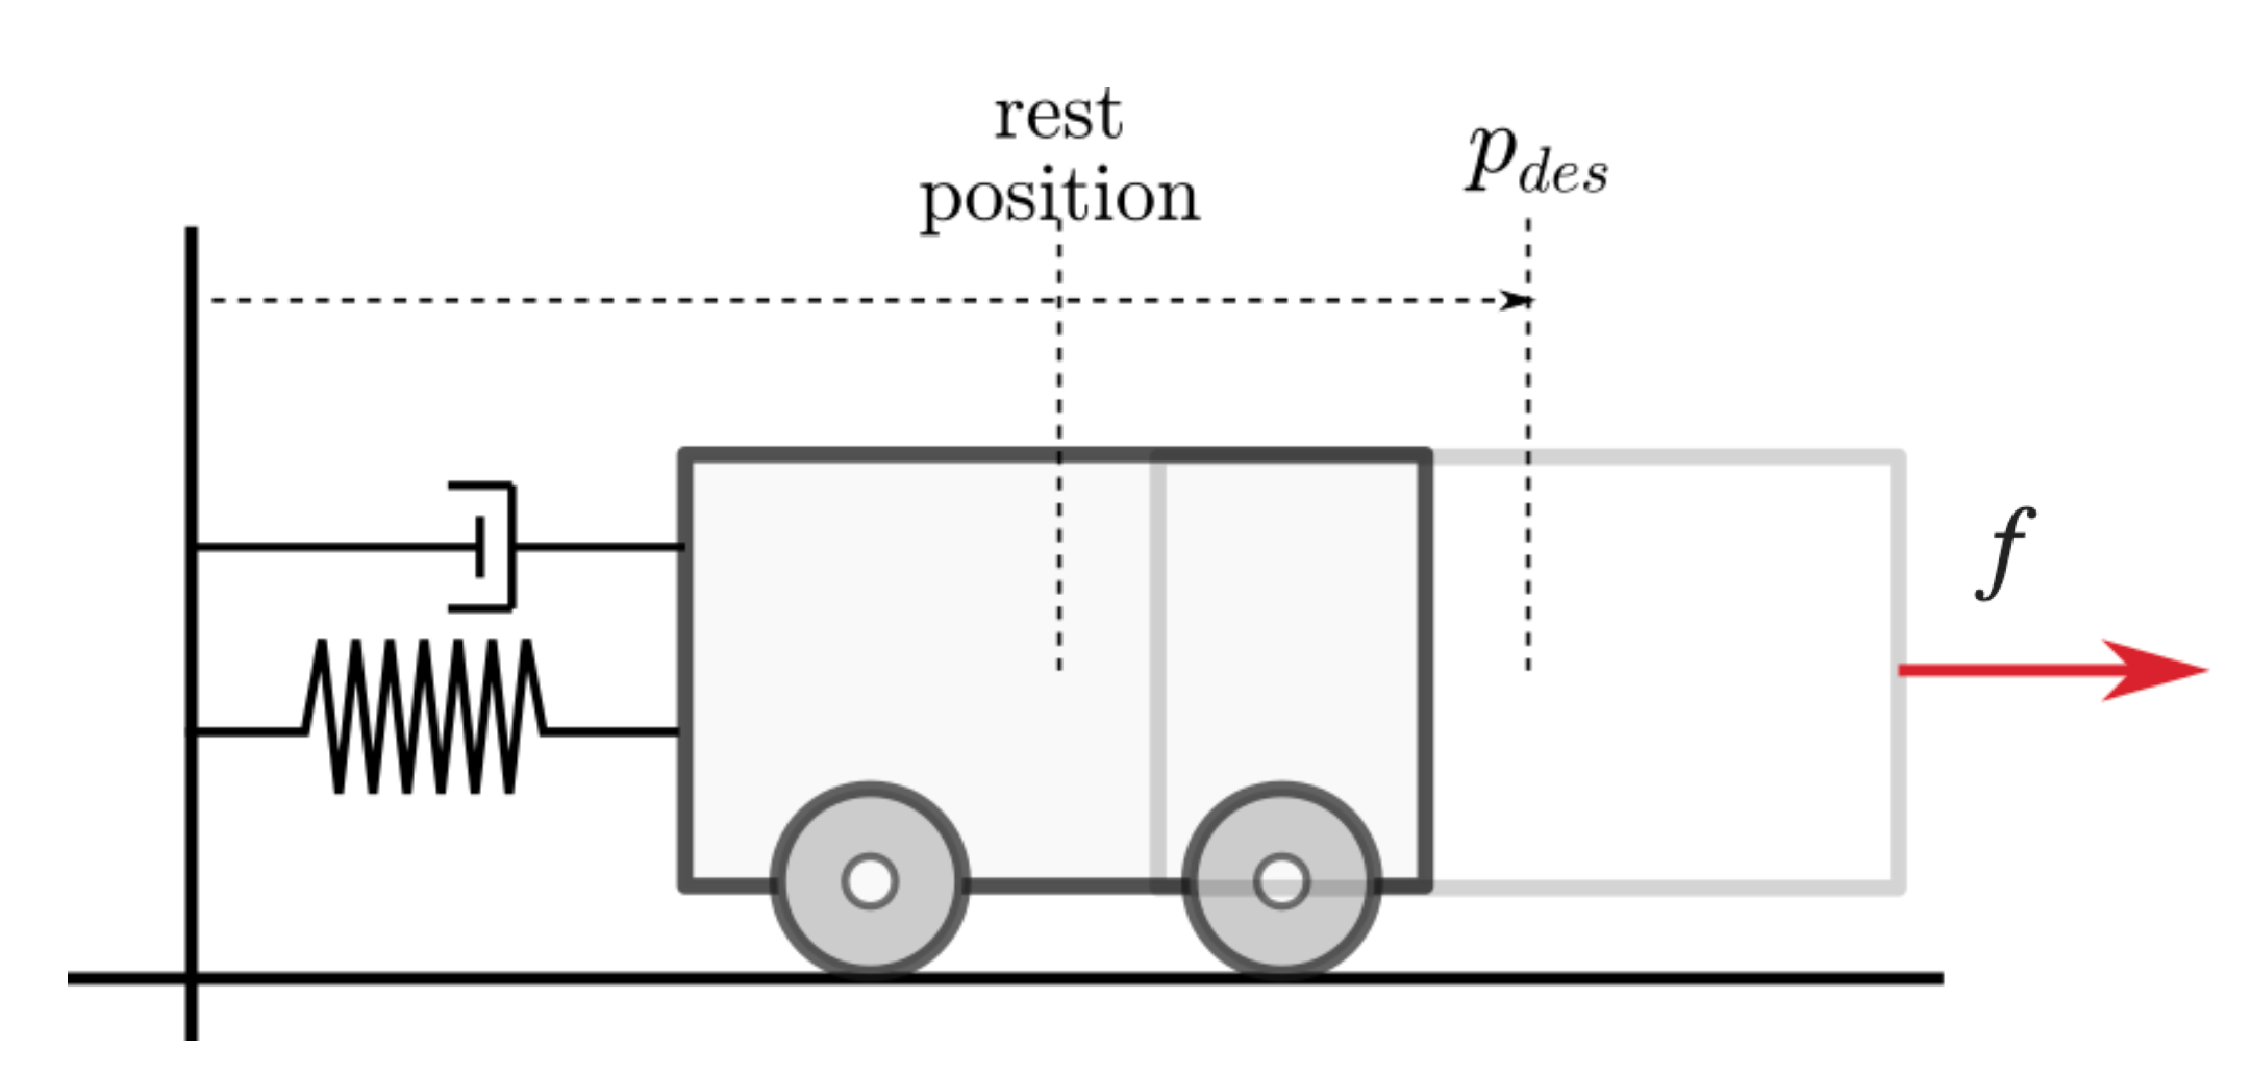
\includegraphics[width=0.5\textwidth]{Figures/fig01.pdf}}

\def\FigureTwo{\centering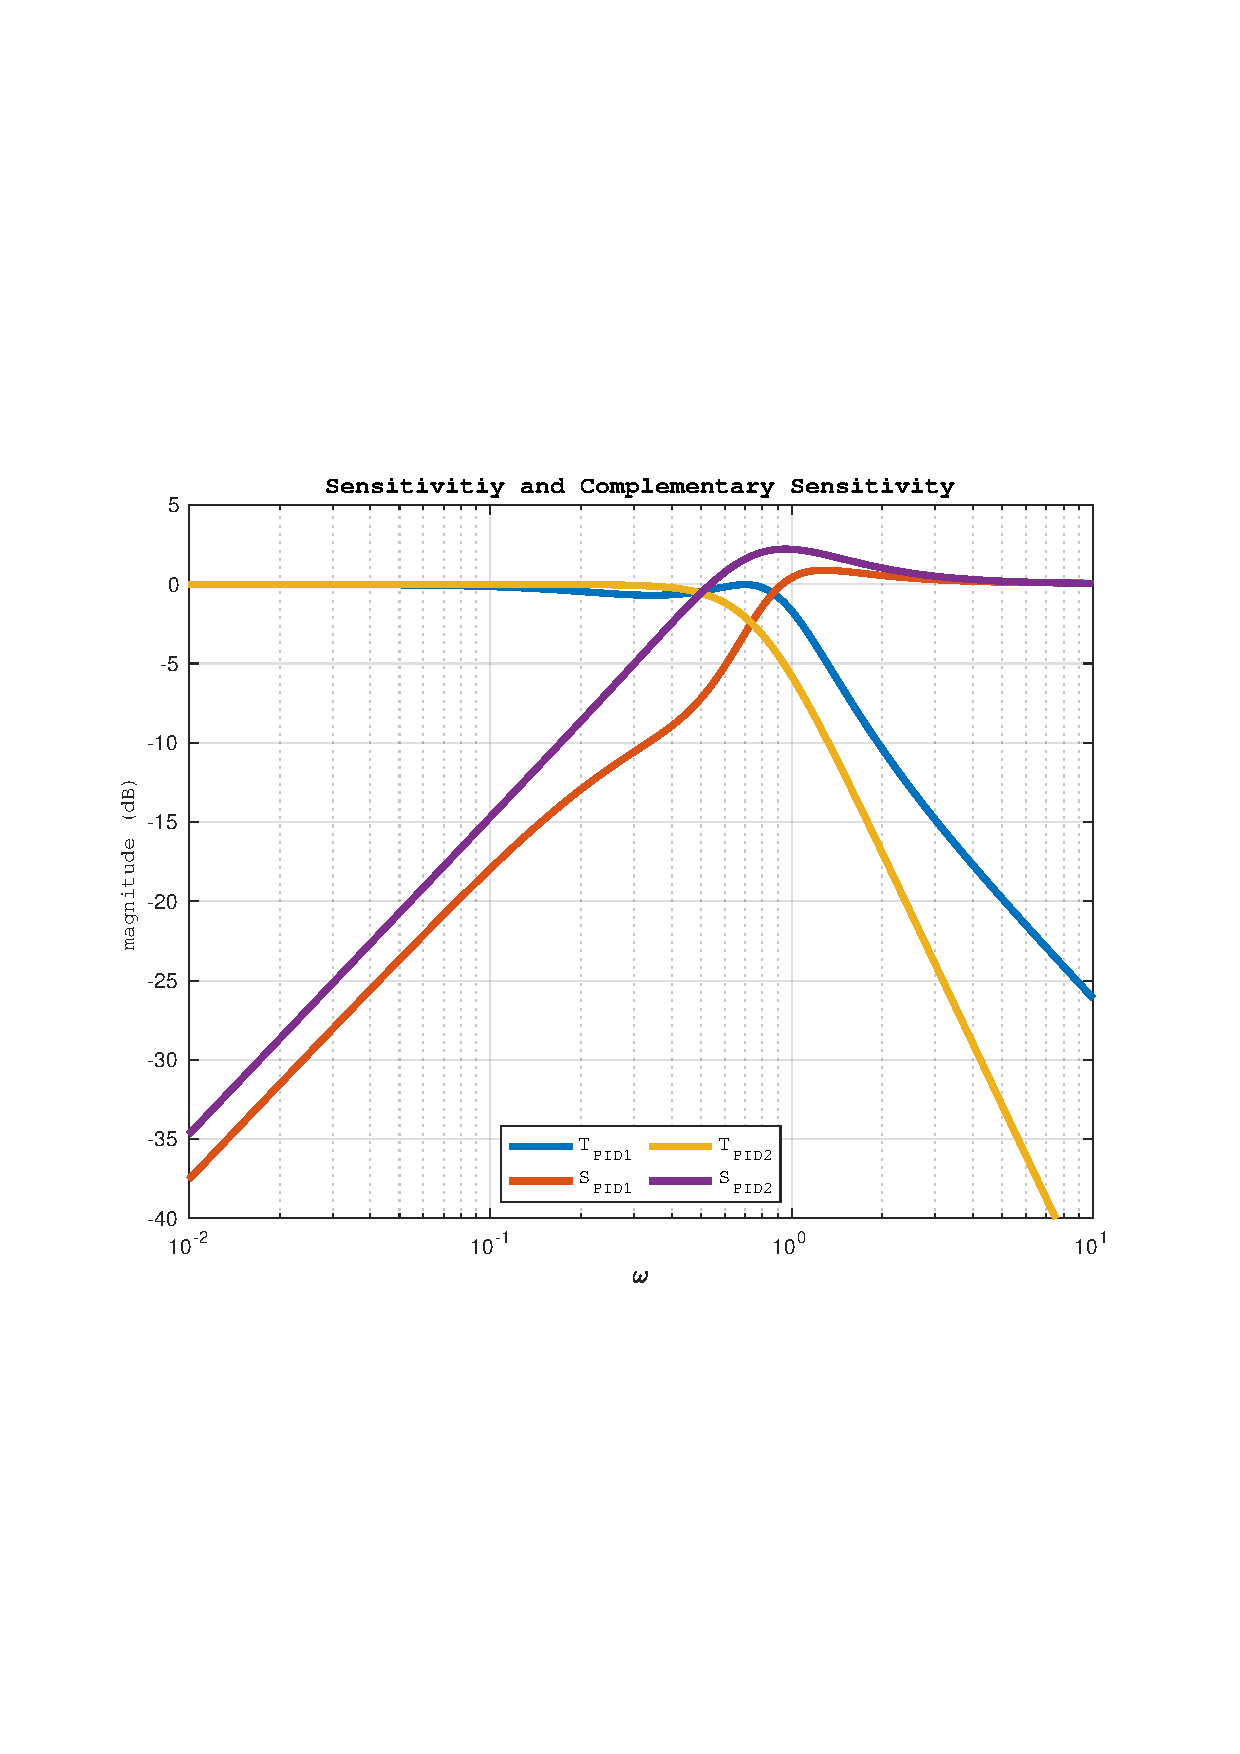
\includegraphics[width=0.5\textwidth]{Figures/fig02.pdf}}

\def\FigureThree{\centering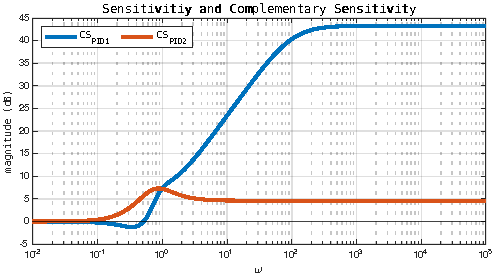
\includegraphics[width=0.7\textwidth]{Figures/fig03.pdf}}

\def\FigureFive{\centering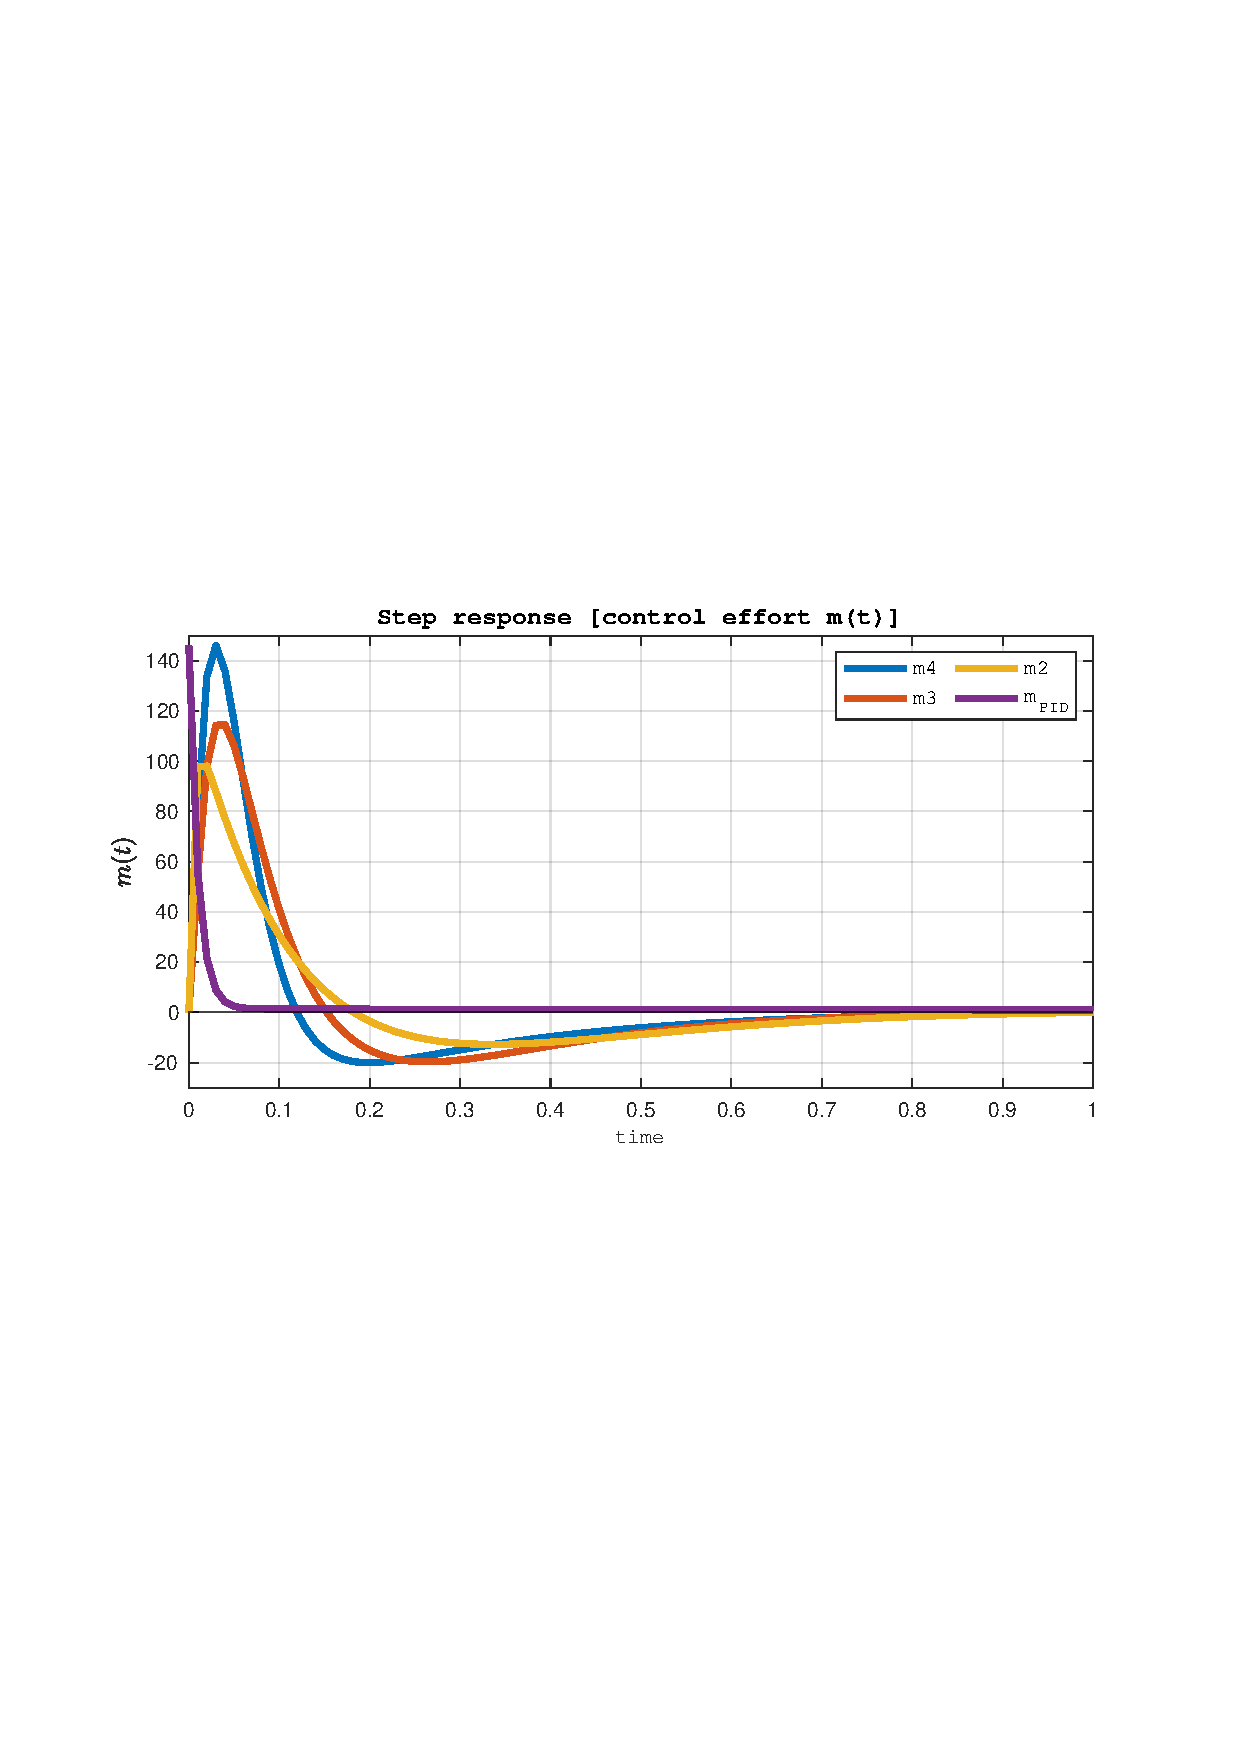
\includegraphics[width=0.8\textwidth]{Figures/fig05.pdf}}


\title{Multivariable Feedback Control \\ Homework 01}
\author{Matteo Scuderi\\ matricola 1937090}
\date{}

\begin{document}

\maketitle

\section{Problem 1: Constant Position Tracking}

In this problem I consider a Mass-Spring-Damper system (from now on, MSD). The goal is to track a desired position $p_{des}$, which for the moment will be assumed constant.\\
To do so, we'll use a 1-DoF $H_\infty$ based control and compare the results obtained with a regular PIDF controller.\\
We'll evaluate our controllers over some classic performance specifications such as, convergence speed, steady state tracking error, transient behavior and  also in terms of noise rejection.

\subsection{Model description and analysis}
\label{sec:ModelDescription}
Consider two plants $MSD_1(s), MSD_2(s)$ based on the same model:
\begin{figure}[h!]
    \FigureOne
    \caption{Visual representation of the MSD model}
    \label{fig:fig01}
\end{figure}

\begin{equation}
        MSD_1(s) = \frac{1}{m_1 s^2 + \mu_1 s + k_1} \qquad  MSD_2(s) = \frac{1}{m_2 s^2 + \mu_1 s + k_2}
\label{eq:Model}
\end{equation}

with all parameters chosen in order to simulate a slightly under-damped and over-damped scenario for the first and second plant, respectively.
\subsubsection*{Remark: Plants' structure}
Both plants are asymptotically stable and minimum phase (best scenario for $H_\infty$ control). However, they both have low bandwidth and therefore also a rather slow response time. The under-damped model, in particular, also presents a (small) resonance peak that will "translate" into a (small) overshoot in the response.
\subsection{Baseline PIDF Controllers}
\label{sec:PIDControllers}

As previously mentioned, I'll use a PIDF controller as a reference to compare it with the $H_\infty$-based controllers' performance.\\
I'll use two "baseline" controllers $C_{PID1},C_{PID2}$, each one tuned appositely on the respective plant, with a design focus on reference tracking (the tuning is made with Matlab's $pidtune(\dots)$).\\
The resulting controllers are reported below:
\begin{equation}
        C_{PID1}(s) = \frac{146.04 (s+0.73) (s+0.70)}
        {s (s+99.23)} \qquad   
        C_{PID2}(s) = \frac{1.70 (s+0.32)}
        {s}
\label{eq:PIDF Controllers}
\end{equation}
It's worth noticing that at closed loop, all sensitivity functions have low bandwidth, as shown in Fig.~\ref{fig:fig02}.
\begin{figure}[h!]
    \FigureTwo
    \caption{Sensitivity and Complementary sensitivity of the two closed loop systems with PIDF controllers}
    \label{fig:fig02}
\end{figure}
\\It's no surprise that the (exact) tracking only occurs after more than 10 seconds, for both systems. \\\\
Another important aspect to analyze is surely the control sensitivity shapes for both systems.
\begin{figure*}[h!]
    \FigureThree
    \caption*{Control sensitivity comparison of the two closed loop systems with PIDF controllers}
\end{figure*}
The Control Sensitivity Function of the underdamped, PID-controlled system significantly amplifies at high frequency, hence the control effort required by our controller will be large when using a step reference (or any signal with high frequency content).
\\
On the other hand, thanks to the high damping, the Control Sensitivity Function for the second system behaves very well and we expect lower control effort, even assigning references with high frequency content.
\\
From a control standpoint, the under-damped system represents a "bigger challenge", having a more oscillating transient and a slower convergence time.
\\\\
For this reason \textbf{I'll base my $H_\infty$ control design exclusively on the first (under-damped) plant} as a further study on the other plant would be an easier and repetitive task.
\clearpage
\subsection{$H_\infty$ based Controllers}
The largest problem with the PID controllers $C_{PID1}(s), C_{PID2}(s)$ is, with no doubt, the slow convergence time. Therefore, my controller design has the \textbf{primary goal of speeding up the response time}, knowing that it will come at a price.\\
\\
Keeping in mind that I'm sacrificing performance in terms of required control effort and high frequency noise rejection, I designed four controllers using the $mixsyn(\dots)$ Matlab function, with the following concept:
\begin{enumerate}
  \item \textbf{$C_1(s)$:} designed with only a sensitivity weight $w_S(s)$ to increase bandwidth.
  \item \textbf{$C_2(s)$:} designed with $w_S$ and a constant control sensitivity bound $K_{S_u}$.
  \item \textbf{$C_3(s)$:} designed with $w_S$ and a control sensitivity weight $w_{S_u}(s)$.
  \item \textbf{$C_4(s)$:} designed with $w_S$, $w_{S_u}$ and a complementary sensitivity weight $w_T(s)$.
\end{enumerate}
with:
\begin{equation}
w_S(s)=\frac{\frac{s}{M_S} + B_{3S}}{s + B_{3S}A_S}
\qquad
w_T(s)=\frac{s+{\frac{B_{3T}}{M _T}}}{A_T\  s+ B_{3T} }
\qquad
w_{S_u}(s)=\frac{s+{\frac{B_{3S_u}}{M_{S_u}}}}{A_{S_u}\  s+ B_{3S_u} }
\label{eq:Weight Functions}
\end{equation}
\subsubsection*{Remark: Choice of the parameters}
The whole list of values chosen can be found in the Matlab file. However, my choice has been consciously very demanding, in order to push the systems at their limit.
Bandwidth for the sensitivity is increased by a factor greater than 10 with respect to the plant's. Sensitivity's module at low frequency is required to be 0.01 whereas at high frequency it shall be under 1.01 (values \textbf{not} in decibel).
\\
\\
The control sensitivity function, on the other hand, has much more "loose" bounds in terms of module, since higher values of control effort are necessary for obtaining faster response speed.
\\
\\
\subsubsection{Controllers Comparison: Sensitivities}
The \textbf{sensitivity functions $S(s)$} are very similar for $C_2, C_3, C_4$ (Fig.~\ref{fig:fig03a}). $C_1$'s sensitivity has the highest bandwidth, which means it's the fastest controller of all, whereas the PID's has significantly lower bandwidth, making it the slowest.
$C_2$'s $S(s)$ presents slightly higher module at low frequency, meaning it will have the largest tracking error of all.
\\\\
The \textbf{complementary sensitivity functions $T(s)$} have (of course) similar peculiarities (Fig.~\ref{fig:fig03b}). The system with $C_1$ will be extremely sensitive to high frequency measurement noise due to high bandwidth, whereas the PID will be quite sound in rejecting it. Among all the others, $C_4$ has a slightly lower bandwidth, thanks to a properly designed weight $w_T$.
\\\\
The price of high bandwidth comes to light in the \textbf{control sensitivity functions $S_u(s)$} comparison (Fig.~\ref{fig:fig03c}). $C_1$'s control sensitivity is not bounded by any weight $w_{S_u}$ and therefore presents a very large peak that translates into extremely high control effort to references with high frequency content. $C_2$'s has the lowest peak of all and therefore I expect a rather good behavior in terms of control effort.
\begin{figure}[h!]
 \begin{subfigure}[t]{0.32\textwidth}
    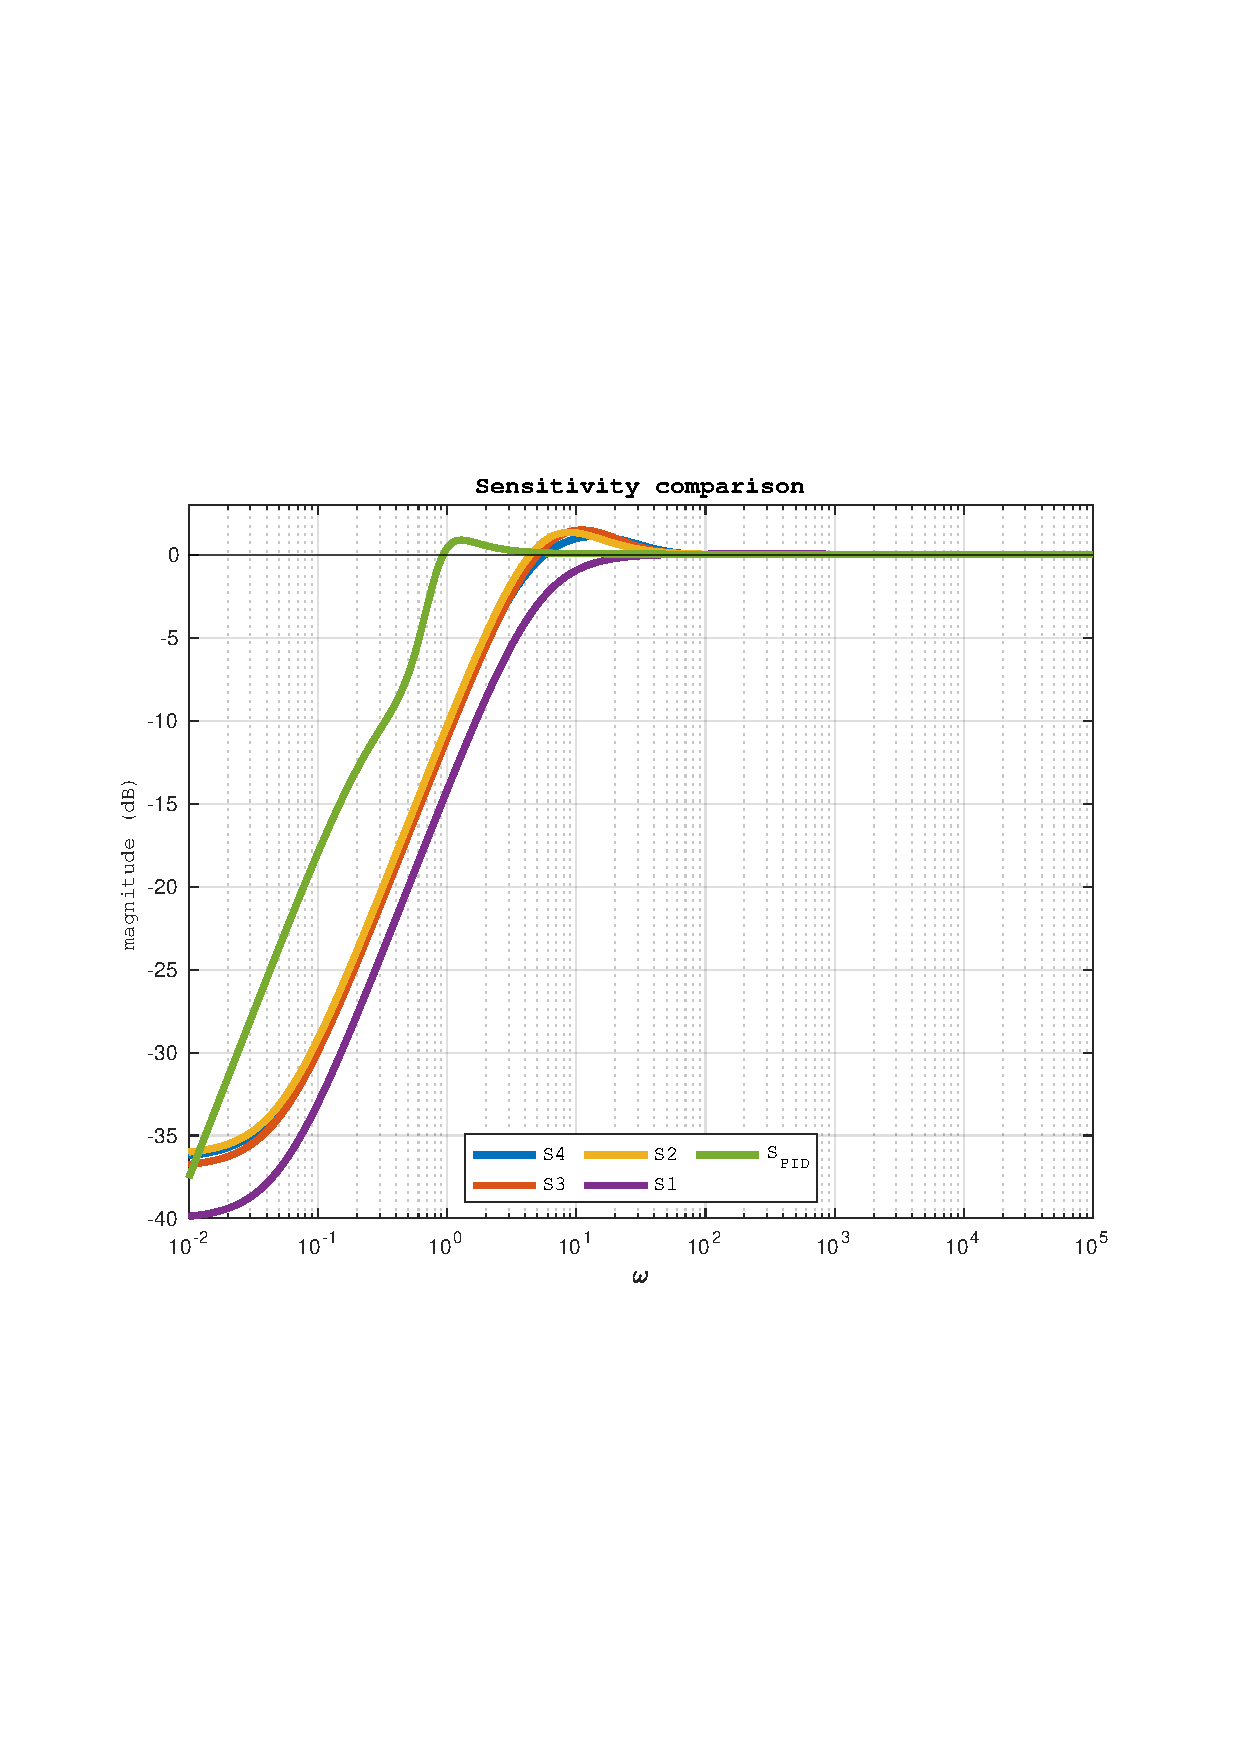
\includegraphics[width=\textwidth]
    {Figures/fig03a.pdf}
    \captionsetup{margin=2mm}
    \caption{$S(s)$ comparison between $H_\infty$ controllers and PID}
    \label{fig:fig03a}
    \end{subfigure}
    \begin{subfigure}[t]{0.32\textwidth}
           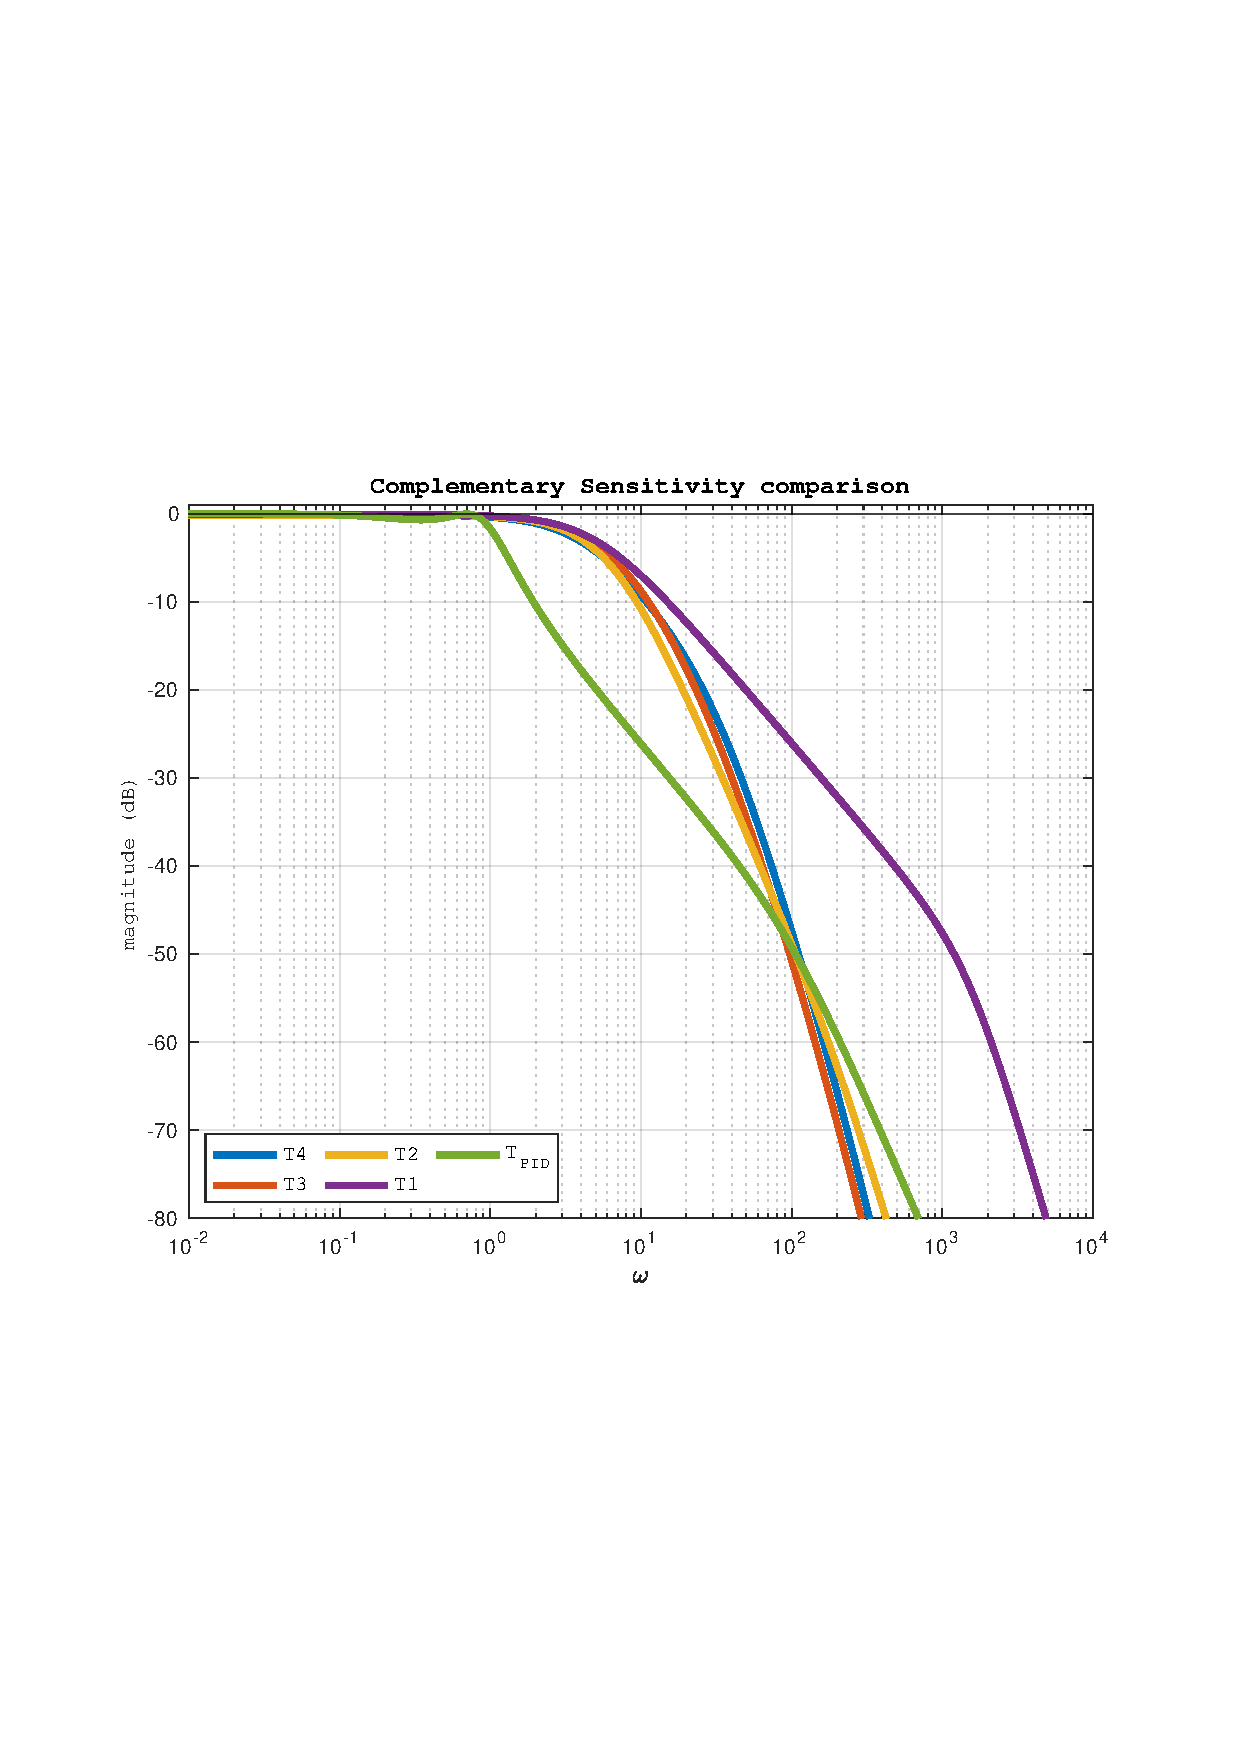
\includegraphics[width=\textwidth]
           {Figures/fig03b.pdf}
           \captionsetup{margin=2mm}
           \caption{$T(s)$ comparison between $H_\infty$ controllers and PID}
           \label{fig:fig03b}
       \end{subfigure}
       \begin{subfigure}[t]{0.32\textwidth}
           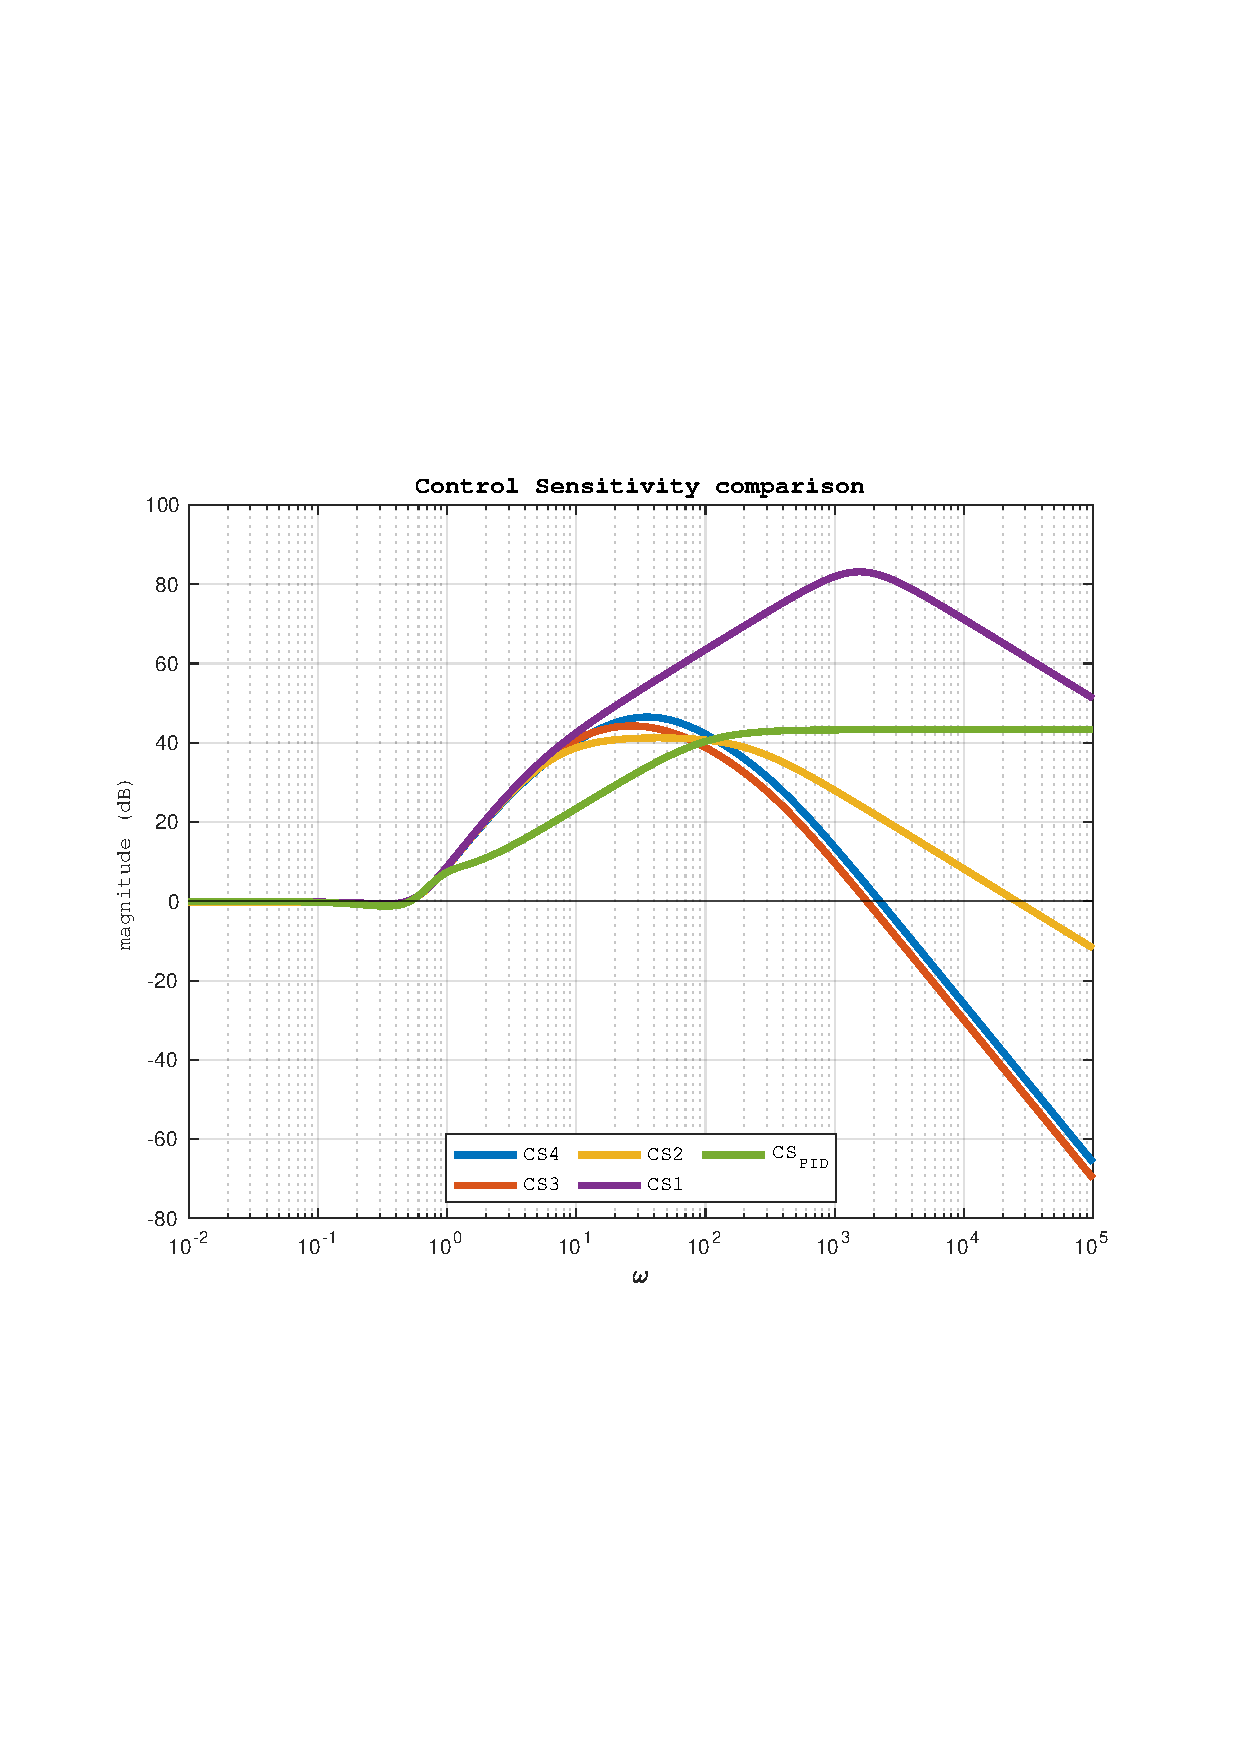
\includegraphics[width=\textwidth]
           {Figures/fig03c.pdf}
           \captionsetup{margin=2mm}
           \caption{$S_u(s)$ comparison between $H_\infty$ controllers and PID}
           \label{fig:fig03c}
       \end{subfigure}
       \caption{Sensitivities comparison between all controllers}
           \label{fig:fig03}
\end{figure}
\clearpage
\subsubsection{Controllers Comparison: Response and Control Effort}
The first controller $C_1(s)$ can only be used as a reference for "ideal behavior". As shown in the Fig.~\ref{fig:fig05}, the control effort required by the other controllers stays between 150$N$ and -30$N$, given a step reference of module one (i.e. a constant desired position $p_{des} = 1$). For $C_1$ there's a peak that goes up to 140.000$N$, which is clearly not realistic.
\\
\\
As a matter of fact, when it comes to reference tracking, $C_1$ has clearly the best performance, displaying a 1\% tracking error and fastest rise time. Fig.~\ref{fig:fig04a}--\ref{fig:fig04b}--\ref{fig:fig04c}.. Keeping that in mind, one can observe similar performances for all other $H_\infty$ controllers.

\begin{figure}[h!]
 \begin{subfigure}[t]{0.8\textwidth}
    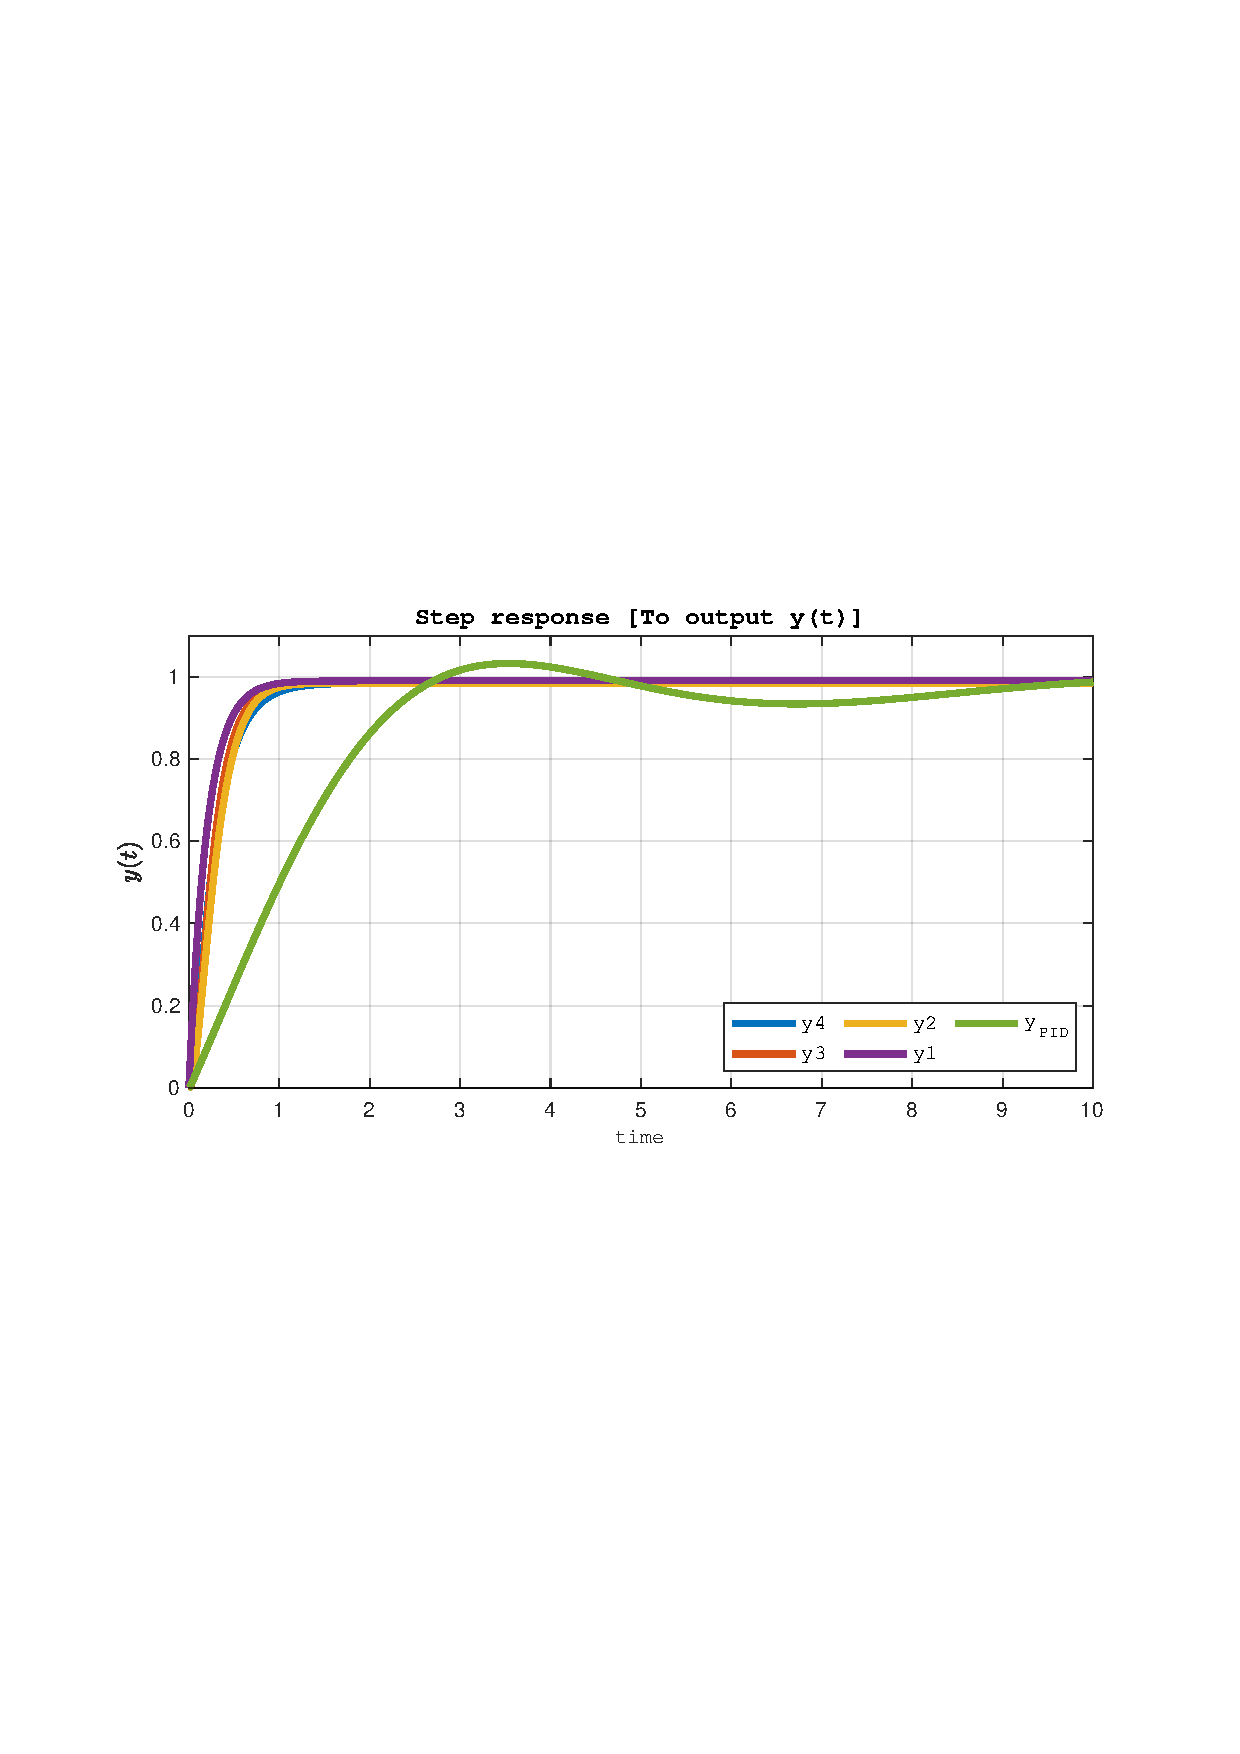
\includegraphics[width=\textwidth]
    {Figures/fig04a.pdf}
    \caption{Step response of the $T_o(s)$ for $C_4, C_3, C_2, C_{PID1}$}
    \label{fig:fig04a}
    \end{subfigure}
    \begin{subfigure}[t]{0.45\textwidth}
           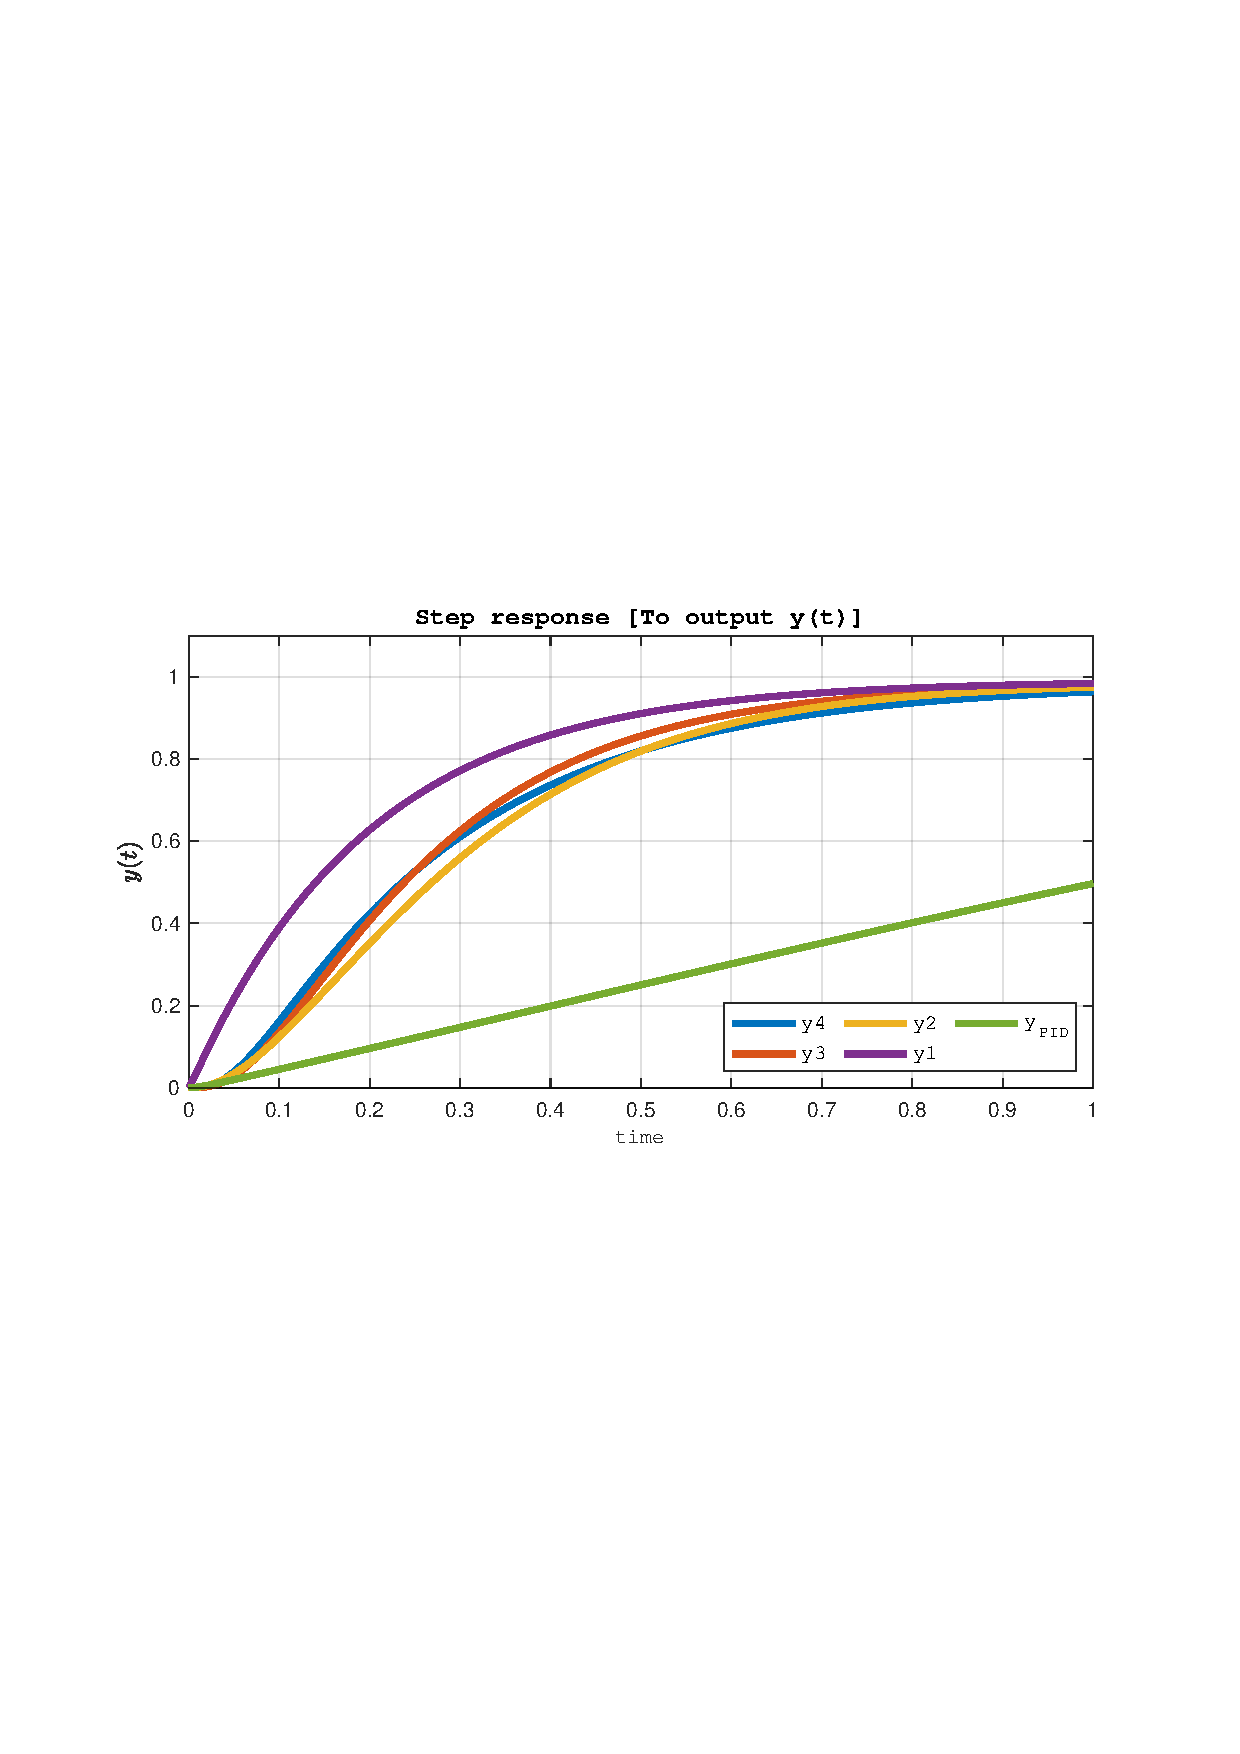
\includegraphics[width=\textwidth]
           {Figures/fig04b.pdf}
           \caption{Transient behavior (zoom in)}
           \label{fig:fig04b}
       \end{subfigure}
       \begin{subfigure}[t]{0.5\textwidth}
           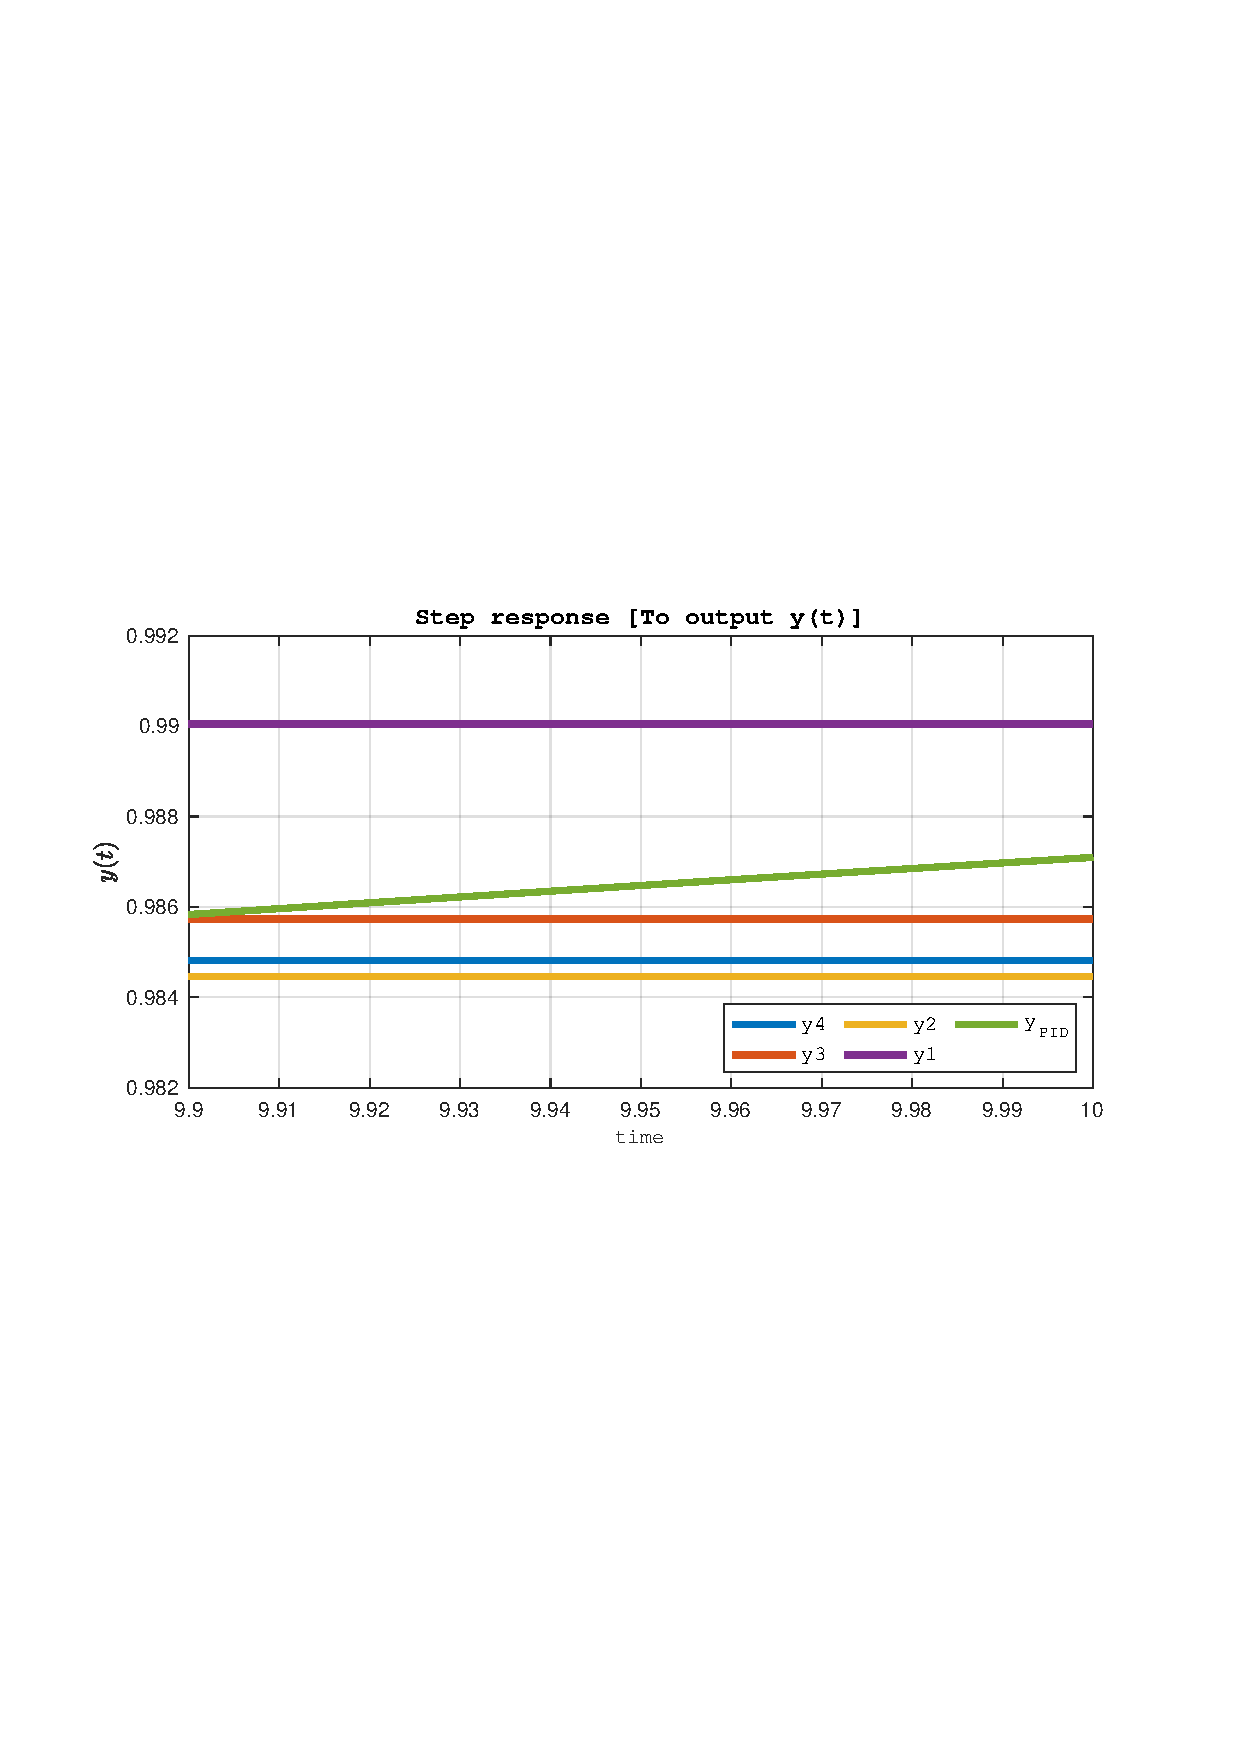
\includegraphics[width=\textwidth]
           {Figures/fig04c.pdf}
           \caption{Steady state behavior (zoom in)}
           \label{fig:fig04c}
       \end{subfigure}
    \label{fig:fig04}
\end{figure}
Fist of all, overshoot has been completely eliminated. Rise time has been more than halved and most importantly, the transient time has been substantially reduced. Notice that at time 10$s$, the PID controller still hasn't converged at $p_{des} = 1$. Tracking error sits -for all $H_\infty$ controllers - below 1.5\%
\begin{figure}[t]
\FigureFive
\caption{Control effort comparison between $C_4, C_3, C_2, C_{PID1}$}
\label{fig:fig05} 
\end{figure}

\subsubsection*{Remark: Plant Canceling}
All $H_\infty$ controllers in use, have a common "shape":
\begin{equation}
    C_i(s) = \frac{\bar C_i(s)}{MSD1(s)}  = 
    (m_1 s^2 + \mu_1 s + k_1)\cdot \bar C_i(s)
\end{equation}
which means each controller is canceling the plant to impose such demanding performances for the sensitivities. This is not at all robust with respect to uncertainties in the parameters, but for this Homework we'll assume a "Perfect" knowledge of our system.

\subsubsection{Conclusion - Problem 1}
The best controller for tracking a constant position, given a step reference is $C_2$. \\Taken $C_1$ and $C_{PID1}$ out of the equation (respectively, unrealistic control effort demand and too slow steady state convergence), the choice must be taken among the other three.
$C_2$ has the largest tracking error, however this is less than 0.2\% more than the other two. On the other hand its control effort demand is 20\% to 30\% less than the above.
\clearpage
\section{Problem 2: Constant Position Tracking - Smooth reference}
One of the problems faced so far involves high frequency content references. Due to the shape of the control sensitivity functions, all controllers react to "rapid reference variations" with rapid control effort increase.\\\\
For this reason, it makes sense to use, instead of a step reference, a smooth version of it that still starts from the rest position and converges to the desired position $p_{des}$. For this purpose, I've tested all the controllers with a sigmoid reference (implementation can be found in the file "$sigmoid\_f.m$").
\\
One way of seeing this is that we've pre-filtered our reference to avoid jumps and attenuate the high-pass-like behavior of the control sensitivity functions.
\\\\
Since I still want fast convergence, I've kept a certain slope to the sigmoid reference, so not to waste all the work done on the controller's "speed".
\\\\
As shown in Fig.~\ref{fig:fig06a}, the tracking is still fast, but most importantly, control effort has been reduced by a factor close to 4 for all $H_\infty$ controllers. (Fig.~\ref{fig:fig06b}). The $C_1$ controller's performance has been left out of the graph since its control effort is still about 20 times larger than $C_2$ (results can be seen in simulink file).\\The PID controller, as suggested by its control sensitivity function, behaves much better with the filtered reference and easily beats all other controllers in terms of control effort (clearly not in transient time, still above 10 seconds).
\begin{figure}[h!]
    \centering
    \begin{subfigure}[b]{0.45\textwidth}
        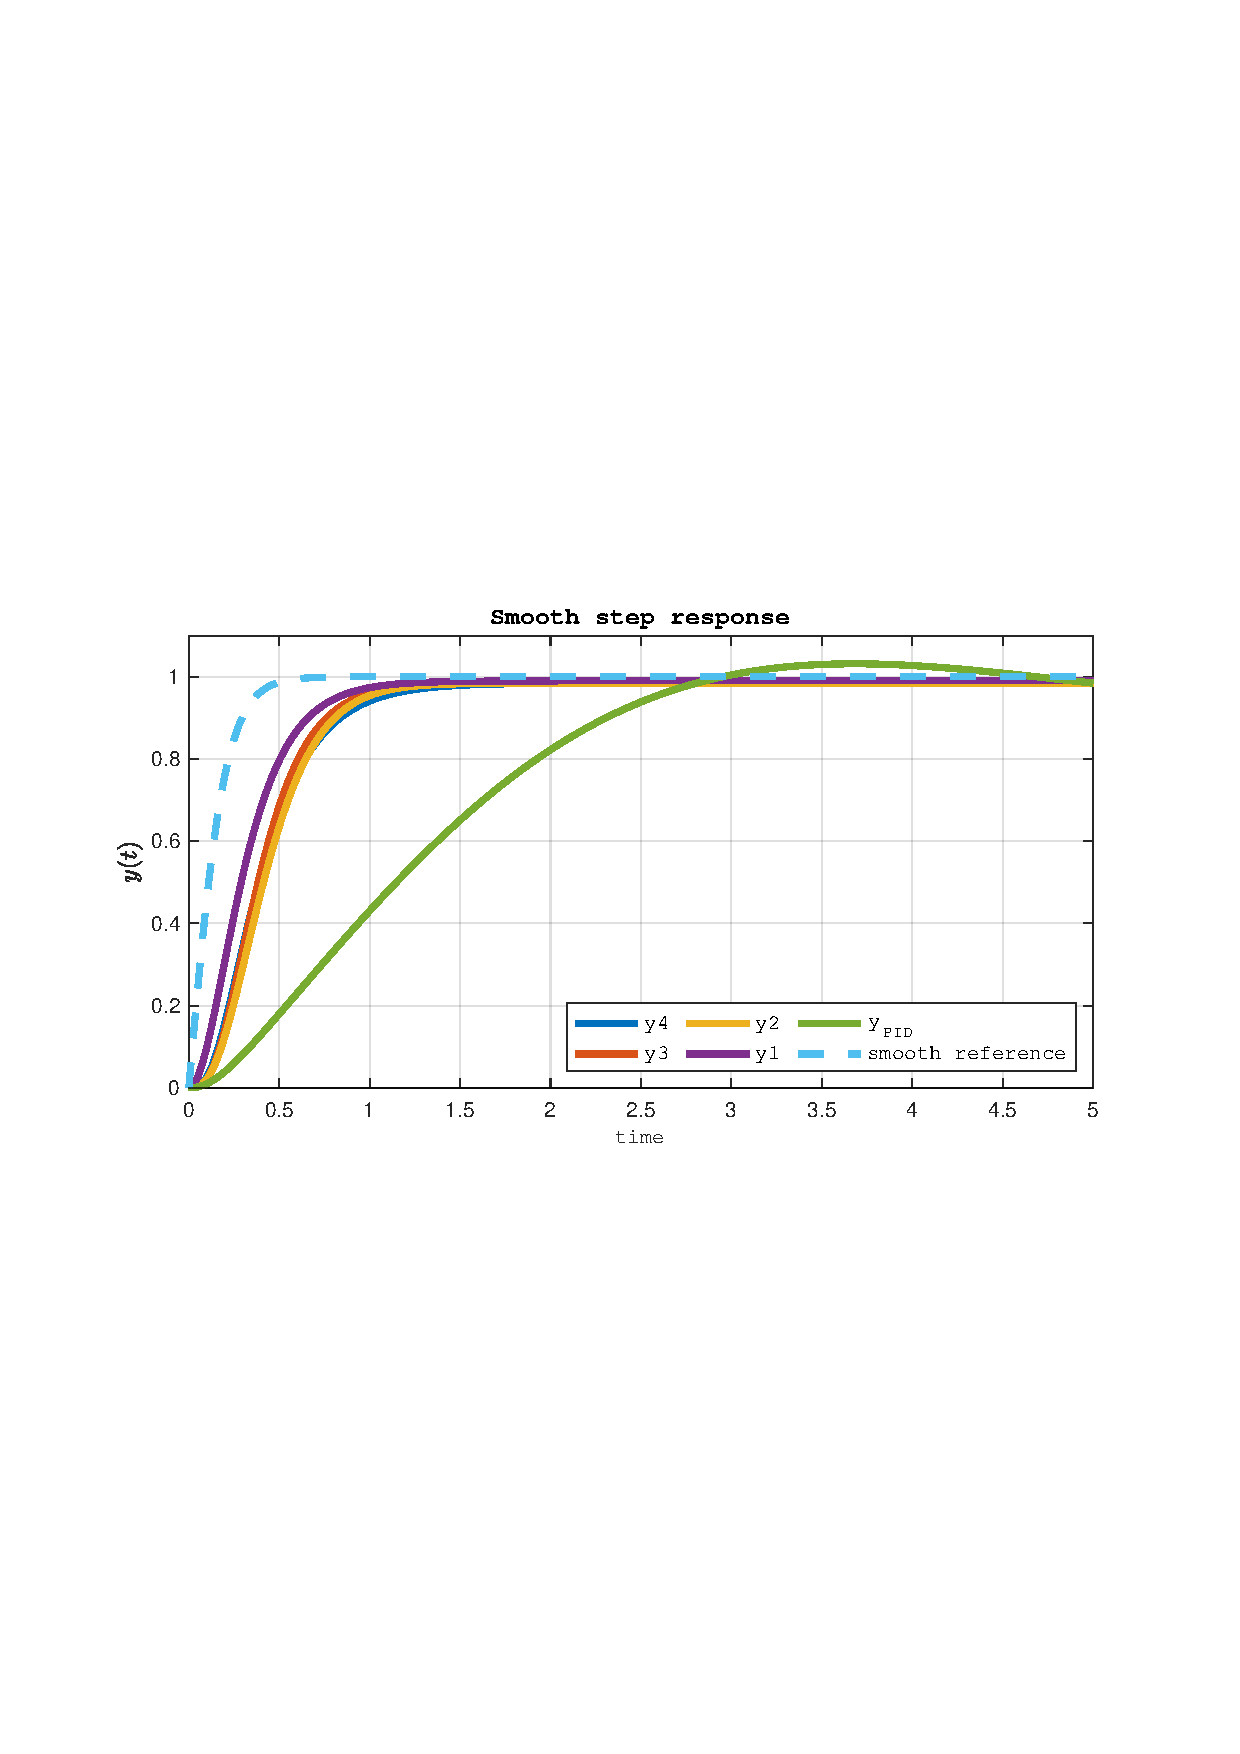
\includegraphics[width=\textwidth]
        {Figures/fig06a.pdf}
            \caption{Position Tracking}
        \label{fig:fig06a}
    \end{subfigure}
    \begin{subfigure}[b]{0.45\textwidth}
        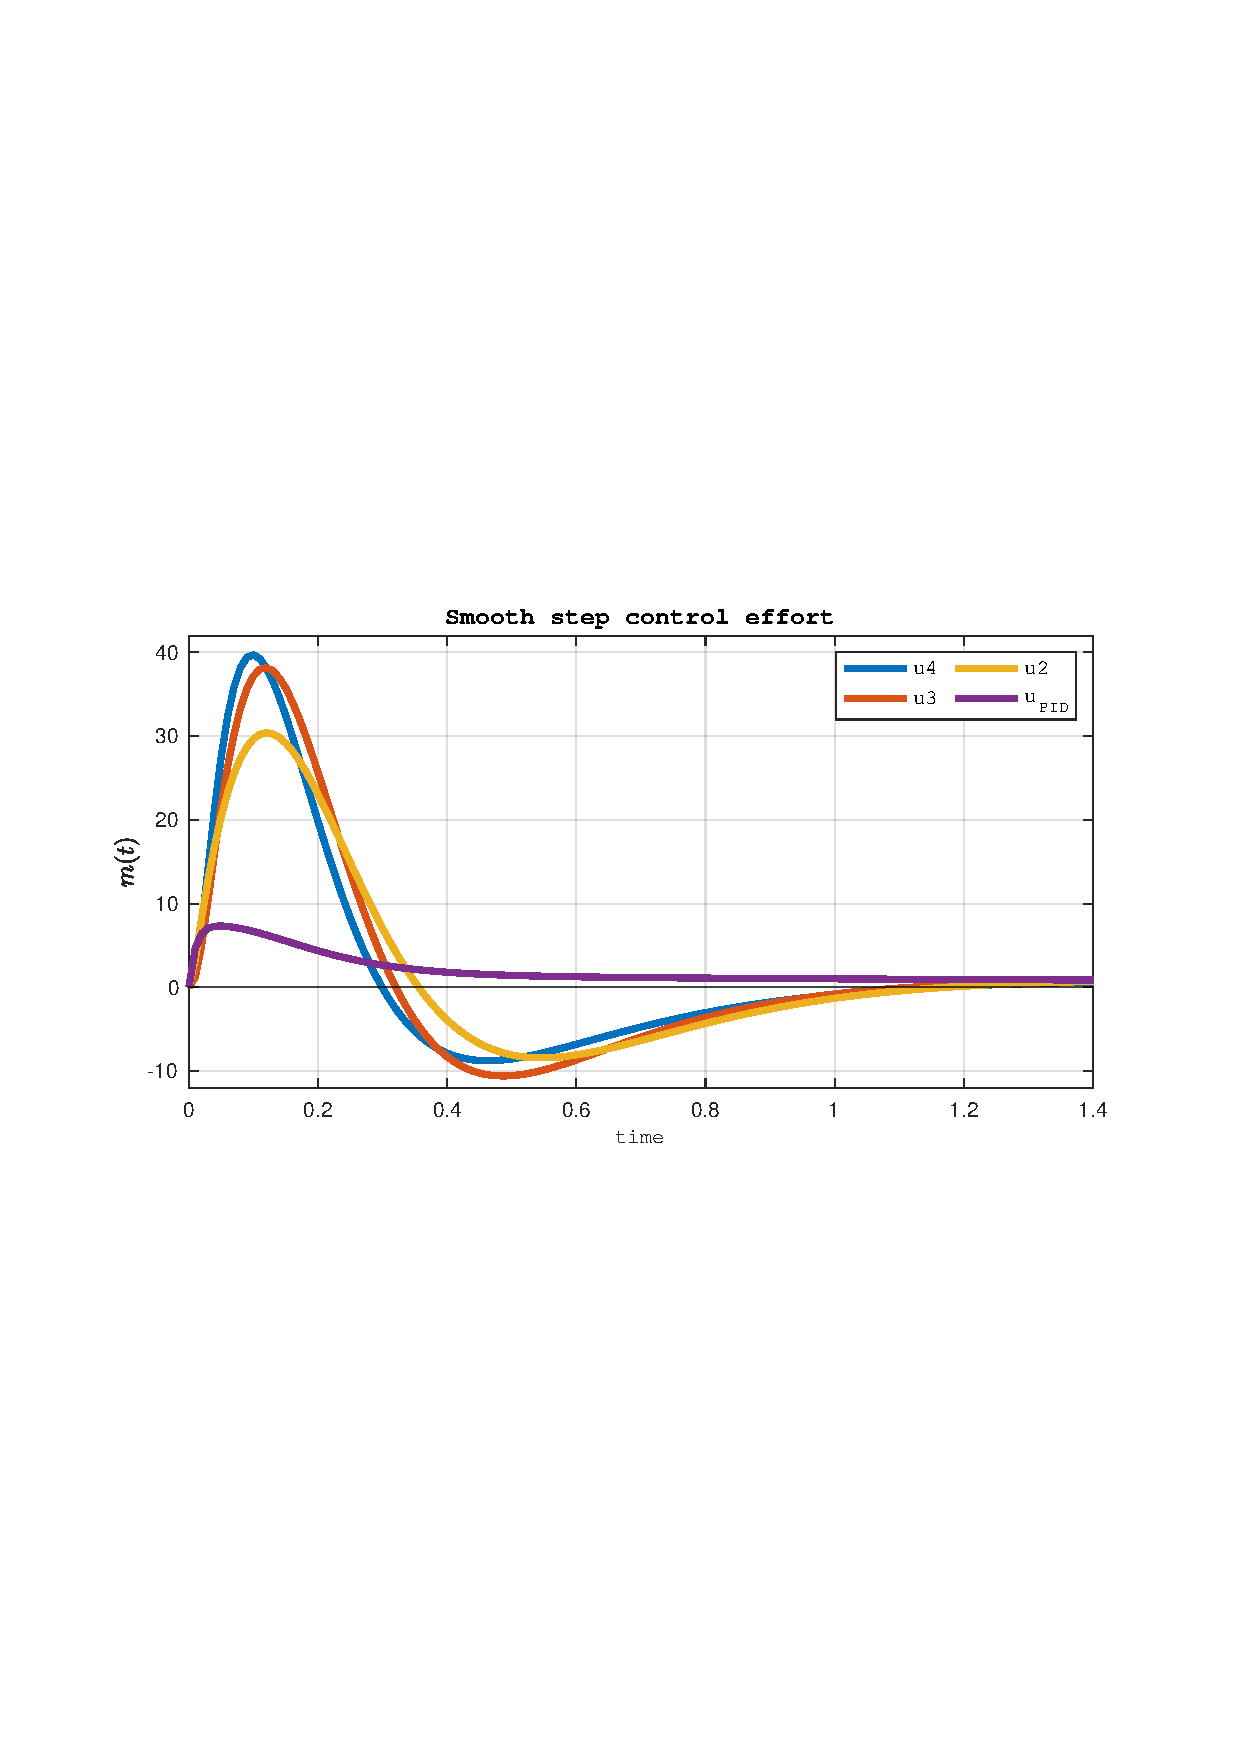
\includegraphics[width=\textwidth]
         {Figures/fig06b.pdf}
        \caption{Control effort}
        \label{fig:fig06b}
    \end{subfigure}
    \caption{Smooth step (sigmoid) system response}
    \label{fig:fig06}
\end{figure}
\clearpage
\subsubsection{Conclusion - Problem 2}
The best controller for tracking a constant position, given a \textbf{filtered} step reference is once again $C_2$. \\
The same remarks hold as for the non filtered case. However, it's worth noticing that with a even milder slope in them reference, the controller $C_1$ could be taken into consideration, as its control effort demand has already dropped significantly. This would still make little to no sense, because it implies sacrificing response speed, which has been the primary goal of the design so far.
\section{Problem 3: Tracking Sinusoidal References}
Looking at the Complementary Sensitivities' modules, it is blatant that tracking sinusoidal references oscillating at medium to high frequency won't be possible. \\As a matter of fact, past a certain frequency, the reference's amplitude will be more and more attenuated, up until total annihilation for high frequencies. Not only that, phase too must be taken into account, as a significant shift translates into relevant errors.
\\To observe this phenomenon, I'll use three sinusoidal references oscillating at frequency [$\omega_1 = 0.1, \omega_2 = 1, \omega_3 = 10$]rad/s.
\begin{figure}[h!]

    \begin{subfigure}[t]{0.50\textwidth}
           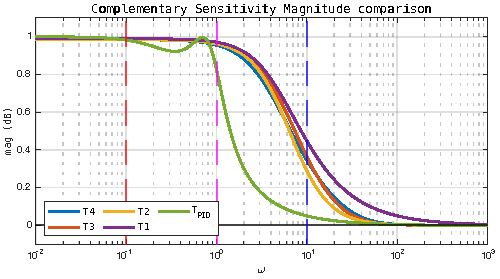
\includegraphics[width=\textwidth]{Figures/fig08a.pdf}
           \caption{T(s) Bode Magnitude comparison}
           \label{fig:fig08a}
       \end{subfigure}
    \begin{subfigure}[t]{0.5\textwidth}
           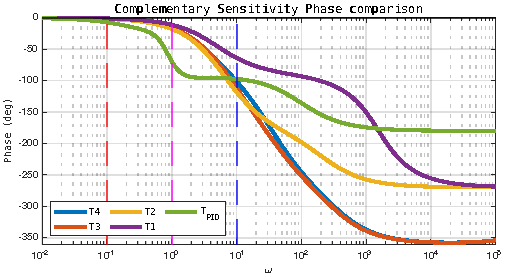
\includegraphics[width=\textwidth]{Figures/fig08b.pdf}
           \caption{T(s) Bode Phase comparison}
           \label{fig:fig08b}
       \end{subfigure}
       \caption{Different attenuation and/or phase shift at each frequency}
    \label{fig:fig08}
   \end{figure}


\begin{figure}[h!]
    \begin{subfigure}[t]{0.60\textwidth}
           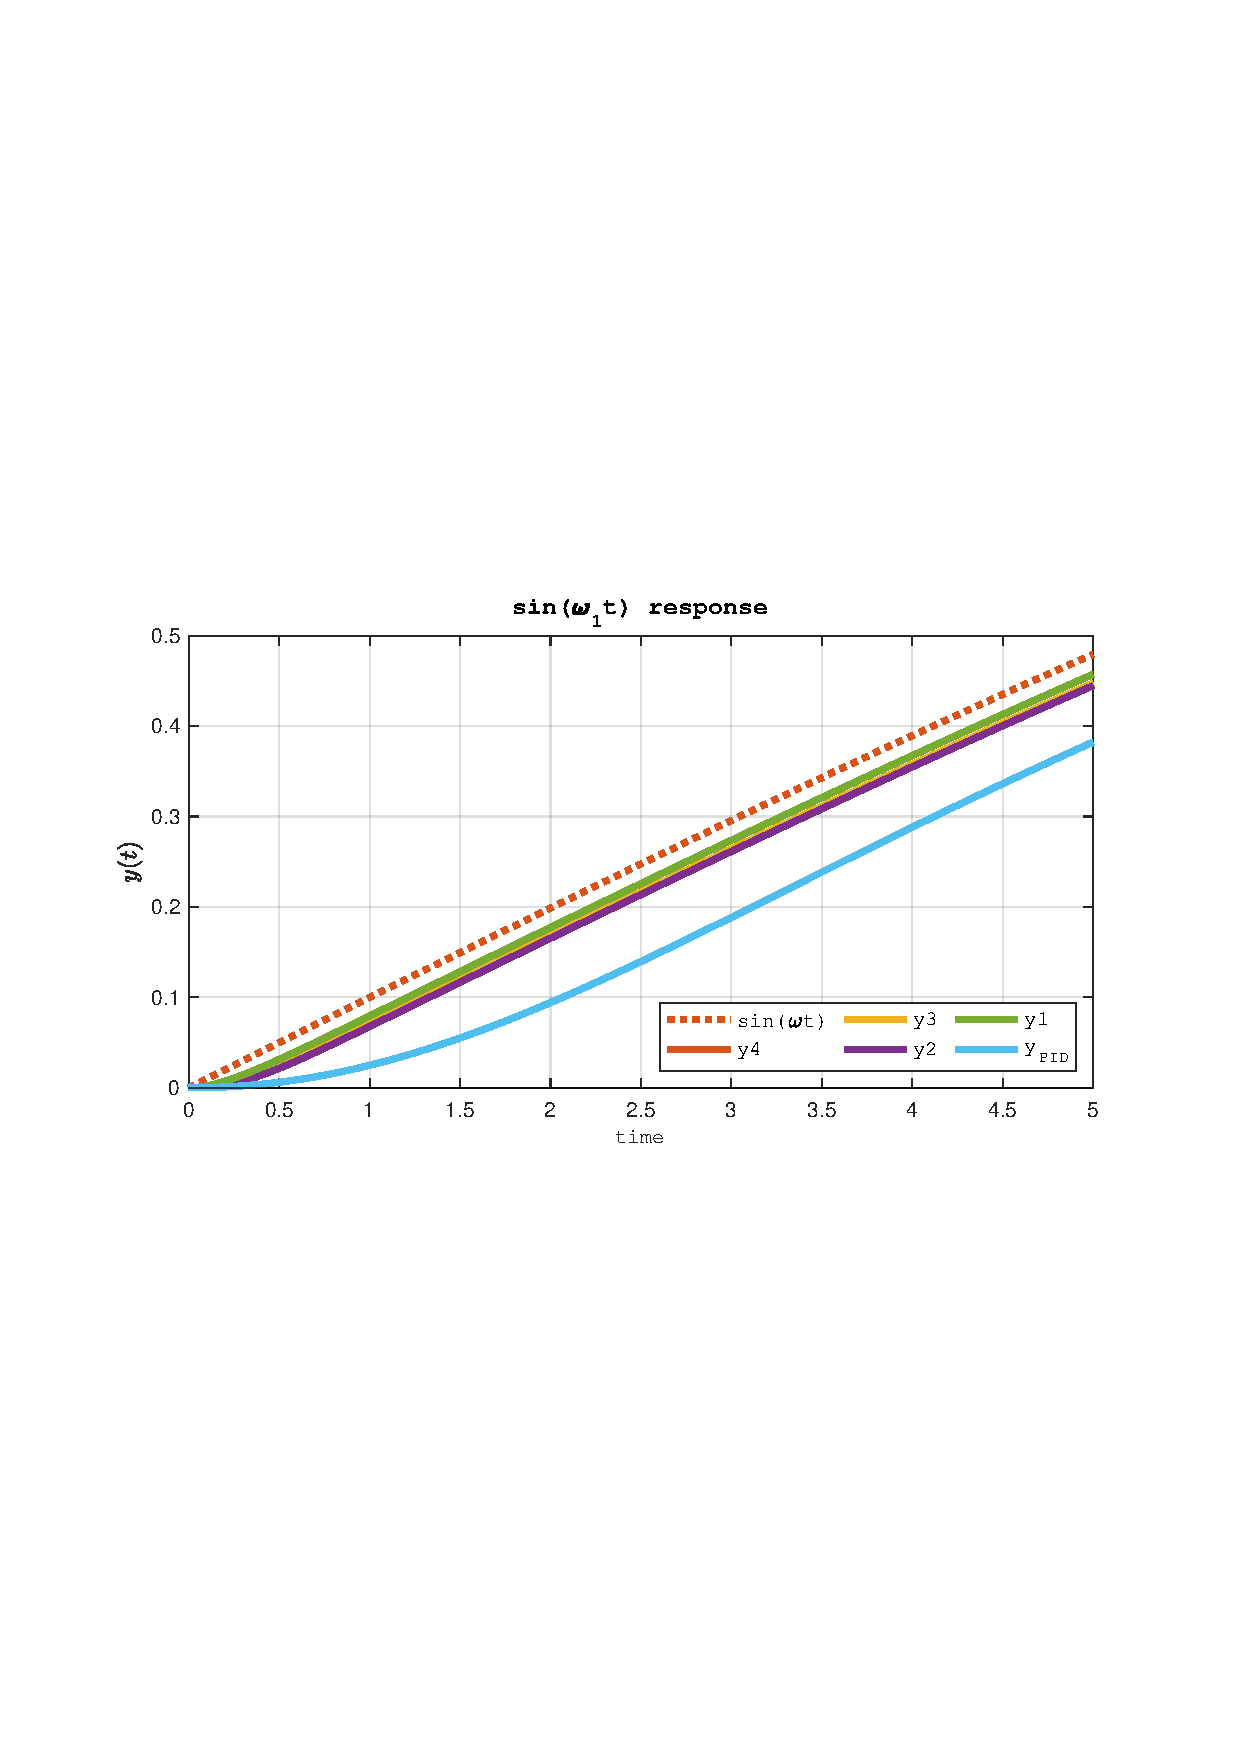
\includegraphics[width=\textwidth]{Figures/fig07a.pdf}
           \caption{Tracking for $\omega_1 = 0.1$}
           \label{fig:fig07a}
       \end{subfigure}
    \begin{subfigure}[t]{0.4\textwidth}
           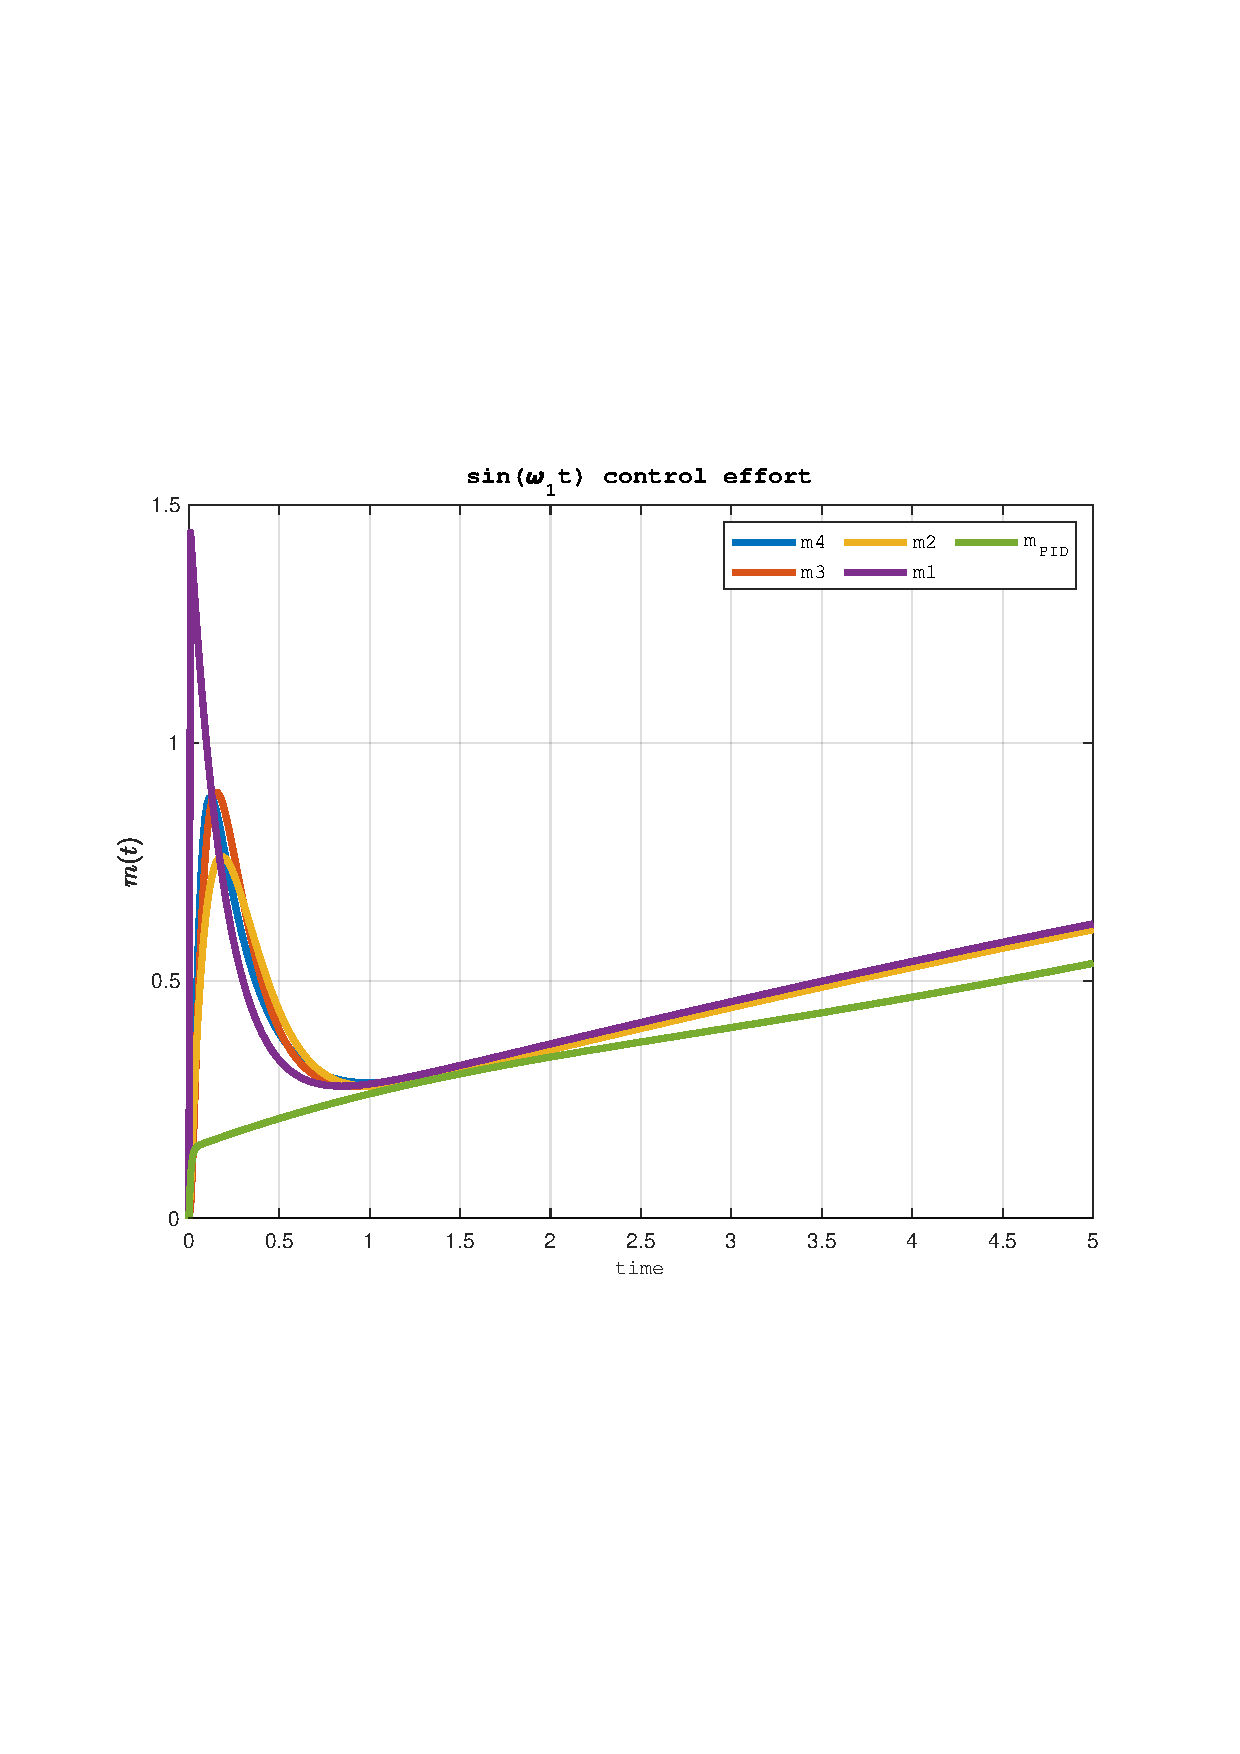
\includegraphics[width=\textwidth]{Figures/fig07b.pdf}
           \caption{Control effort for $\omega_1 = 0.1$}
           \label{fig:fig07b}
       \end{subfigure}
\begin{subfigure}[t]{0.60\textwidth}
           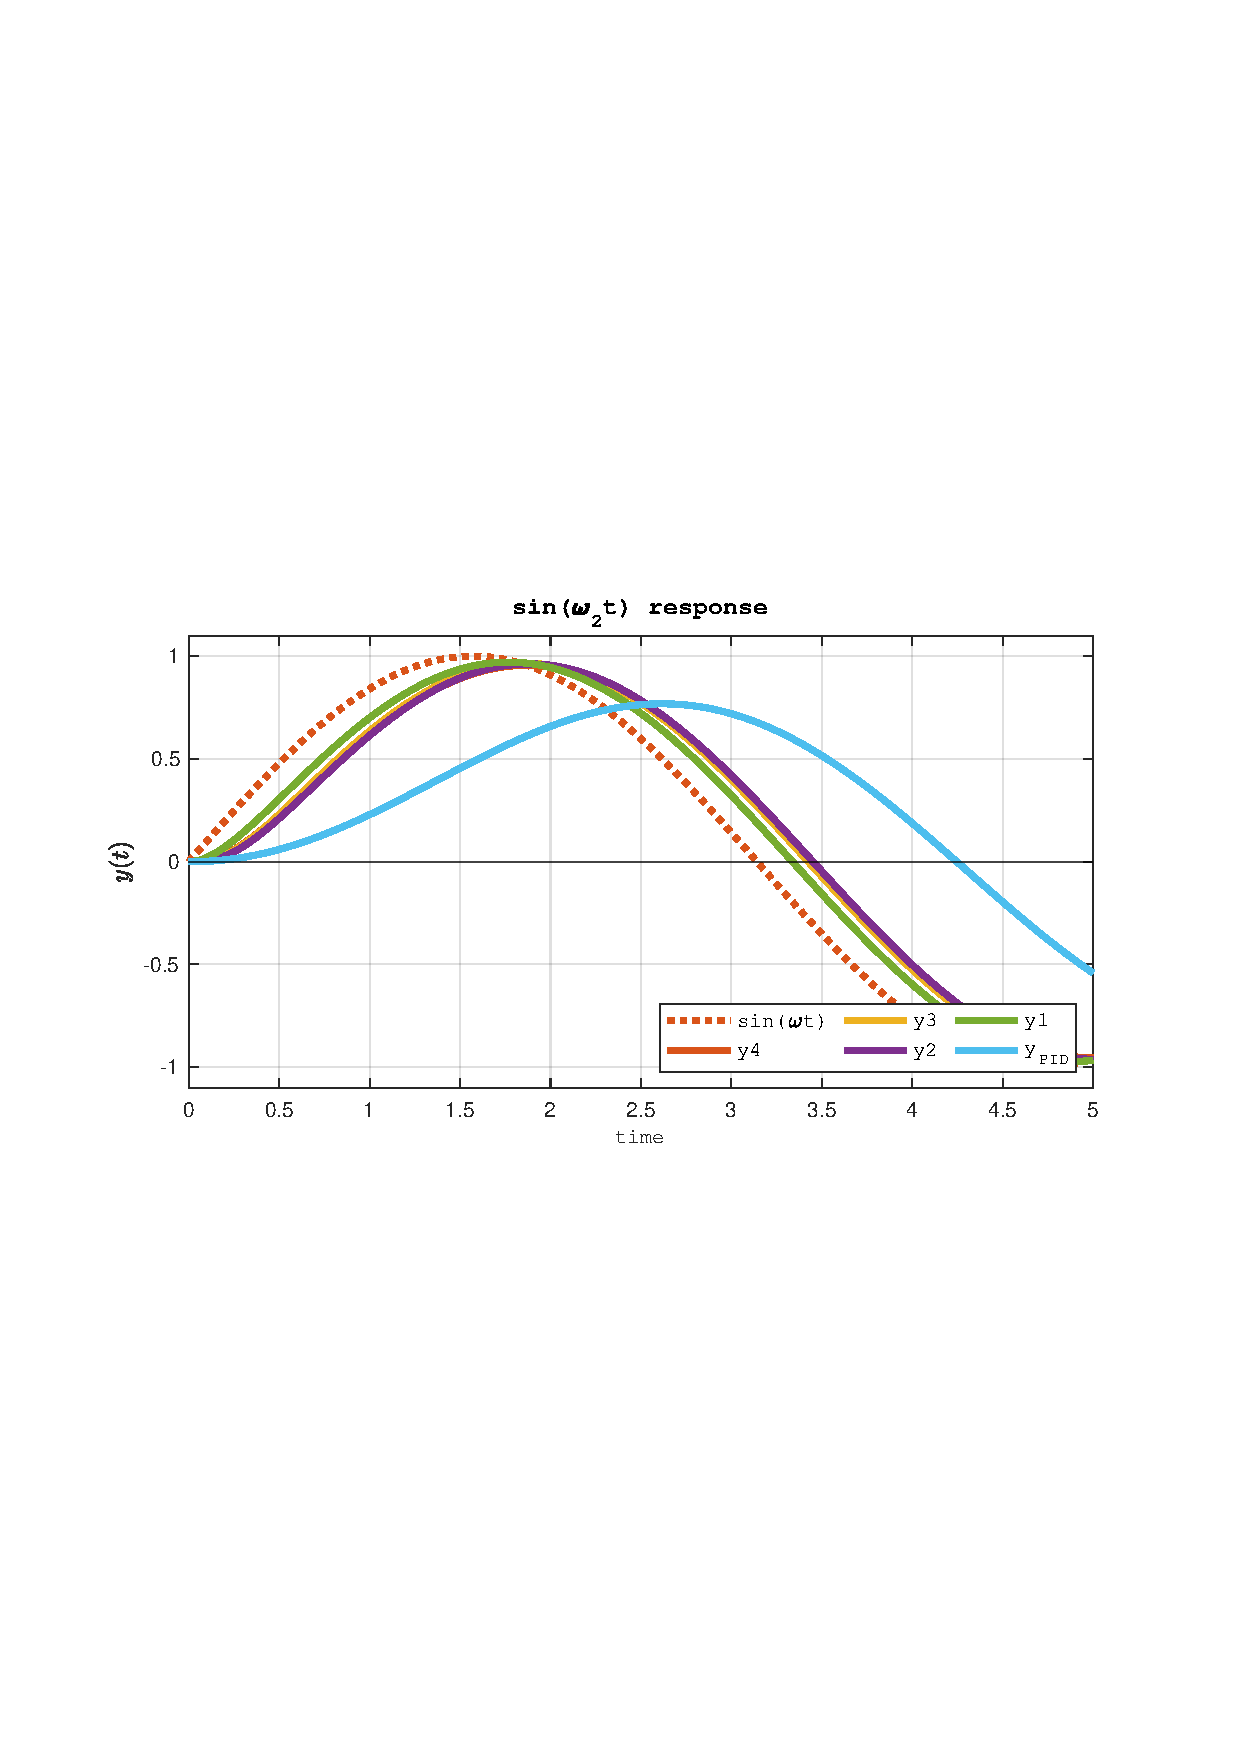
\includegraphics[width=\textwidth]{Figures/fig07c.pdf}
           \caption{Tracking for $\omega_2 = 1$}
           \label{fig:fig07c}
       \end{subfigure}
    \begin{subfigure}[t]{0.4\textwidth}
           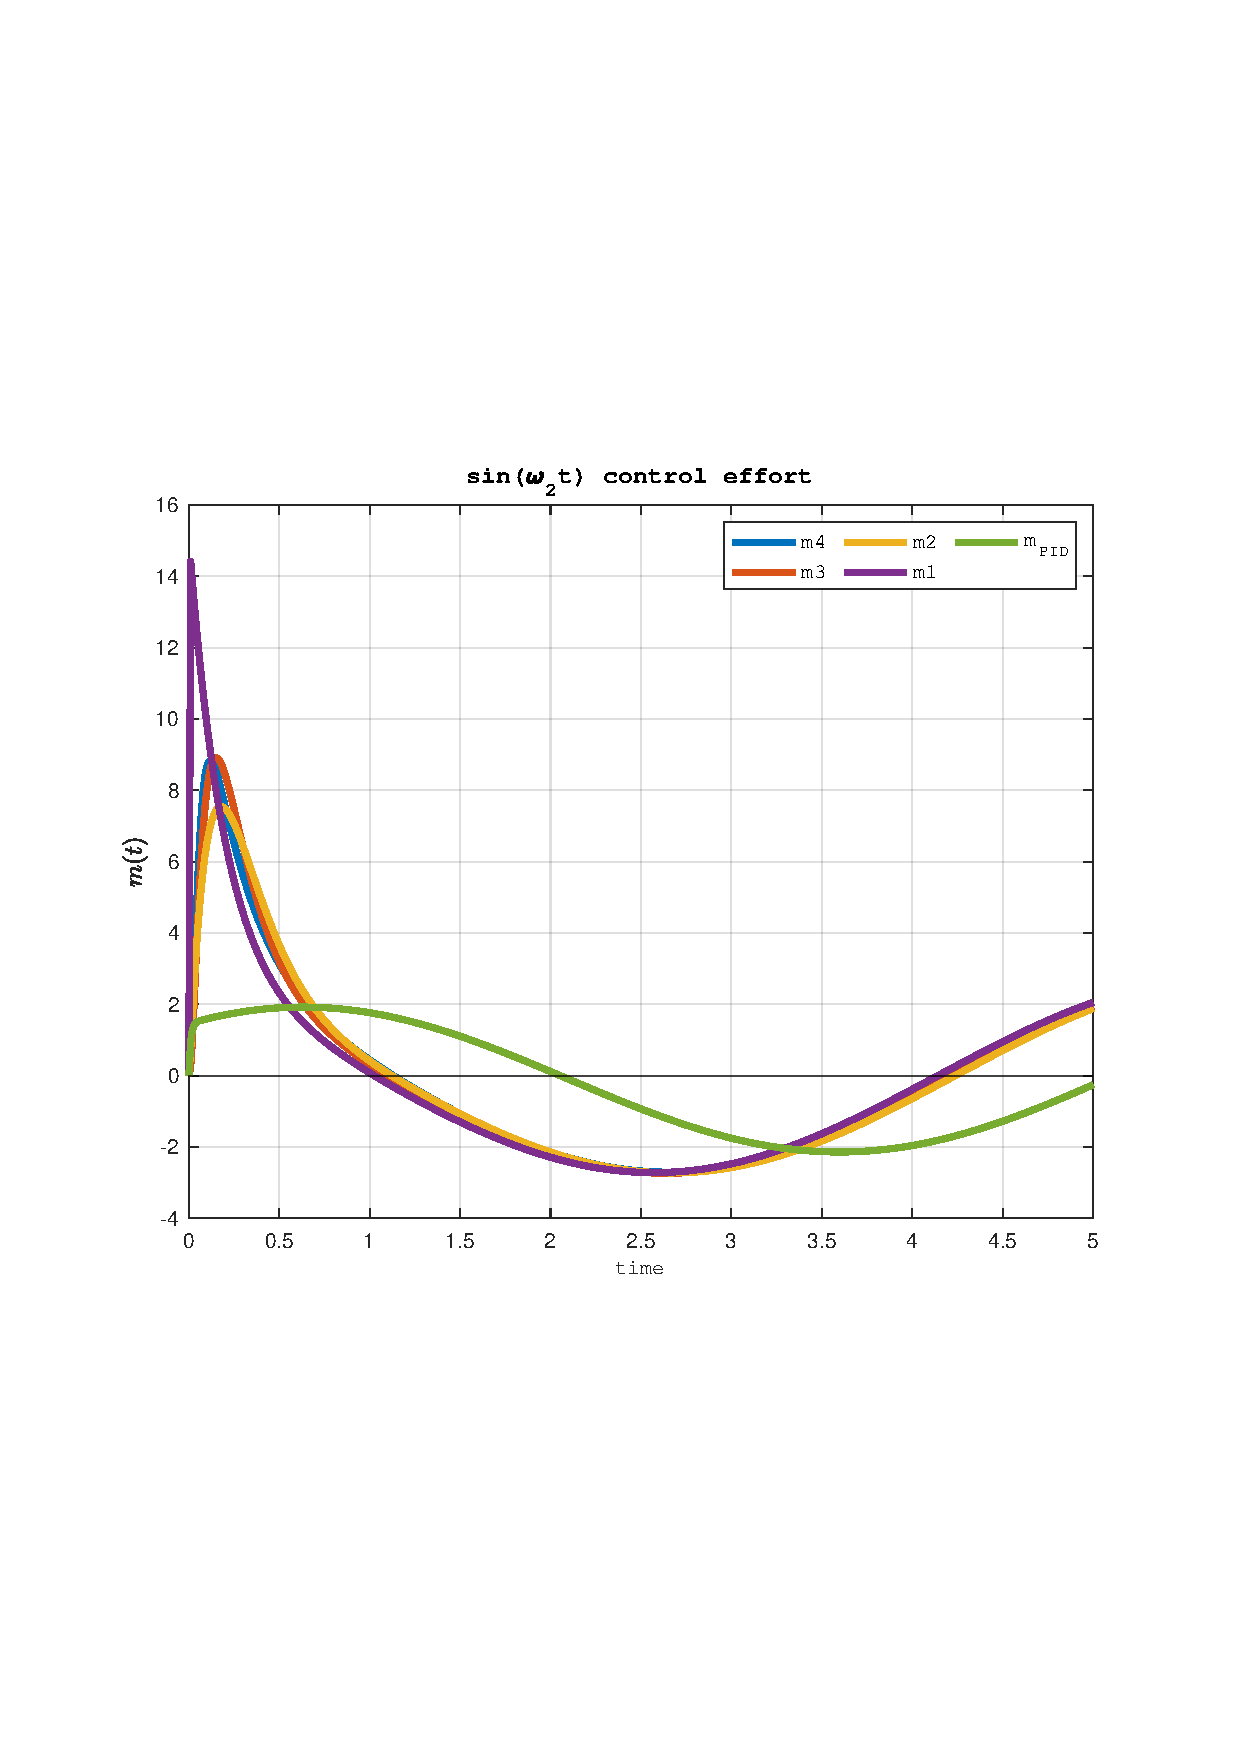
\includegraphics[width=\textwidth]{Figures/fig07d.pdf}
           \caption{Control effort for $\omega_2 = 1$}
           \label{fig:fig07d}
       \end{subfigure}
       \begin{subfigure}[t]{0.60\textwidth}
           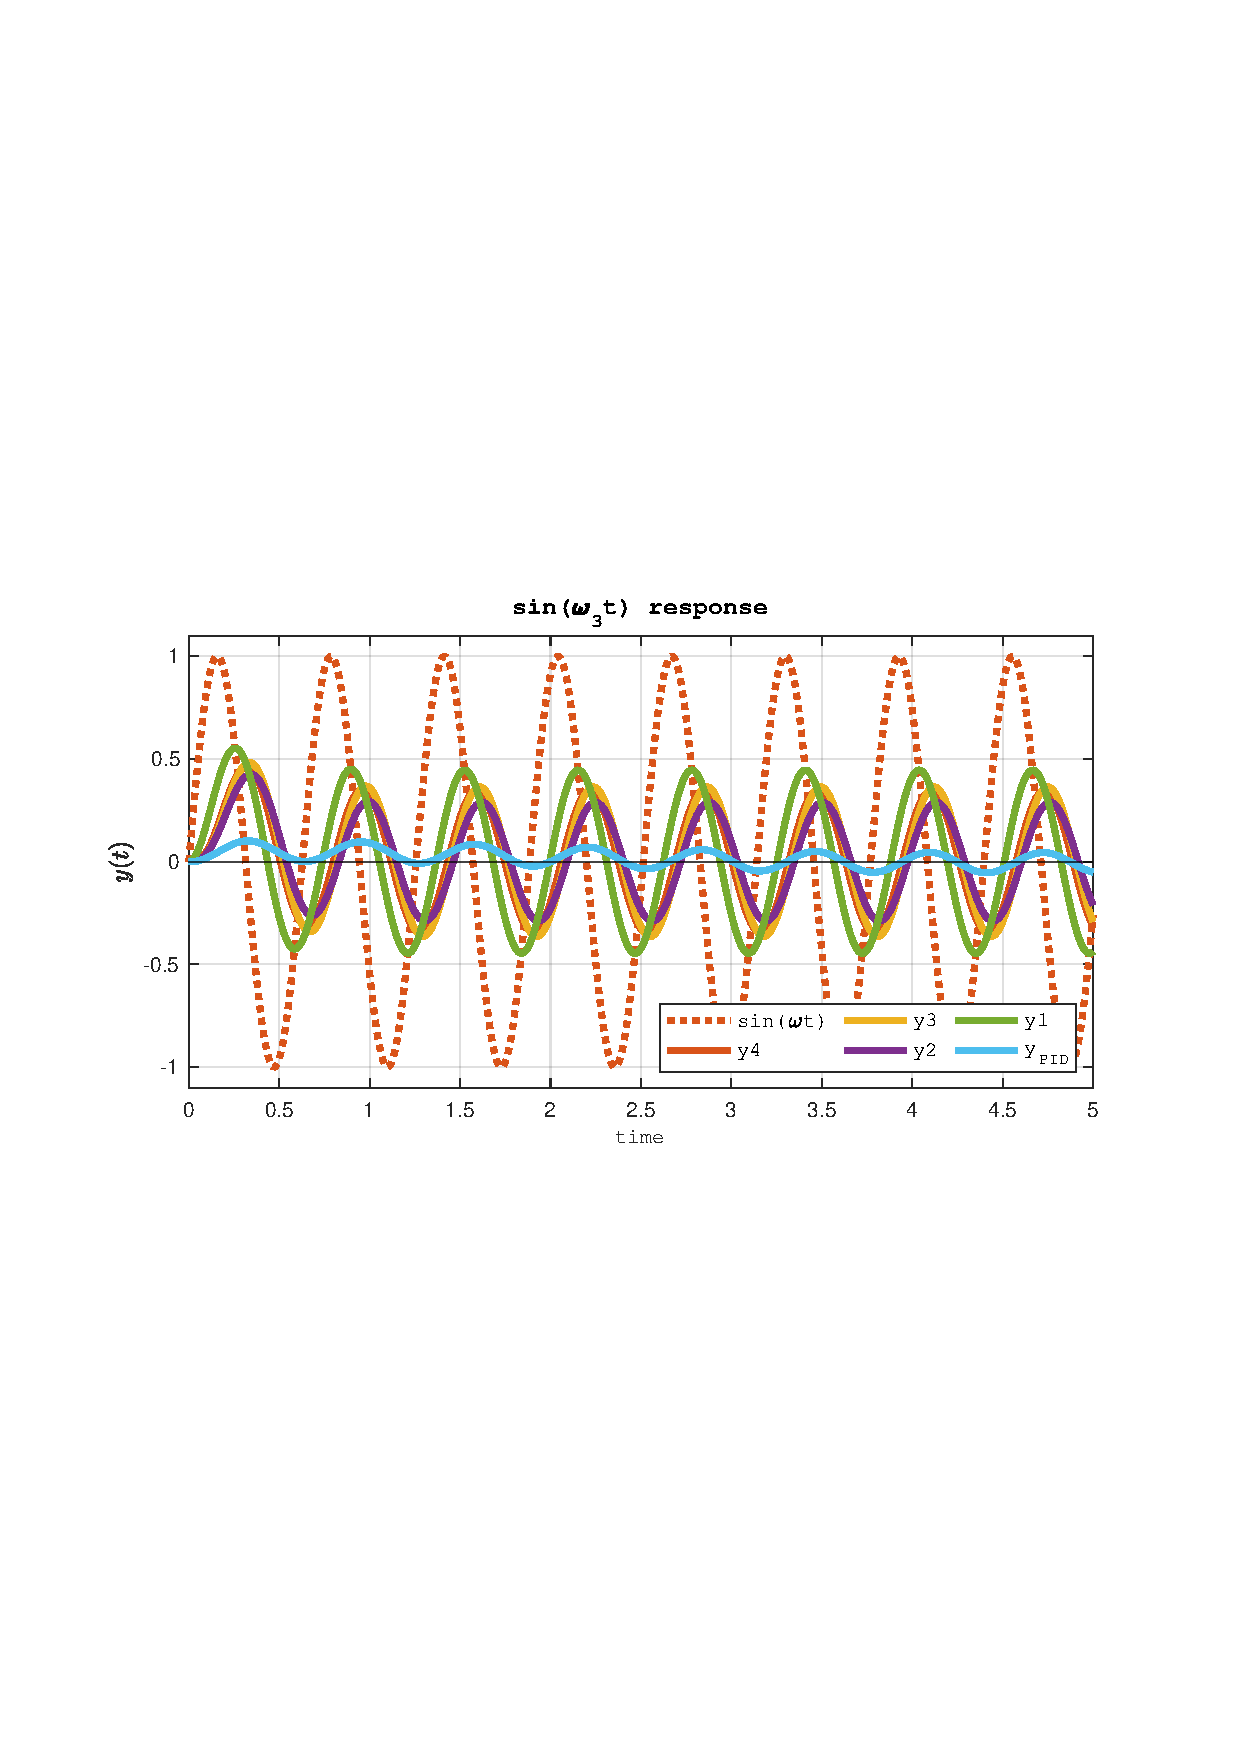
\includegraphics[width=\textwidth]{Figures/fig07e.pdf}
           \caption{Tracking for $\omega_3 = 10$}
           \label{fig:fig07e}
       \end{subfigure}
    \begin{subfigure}[t]{0.4\textwidth}
           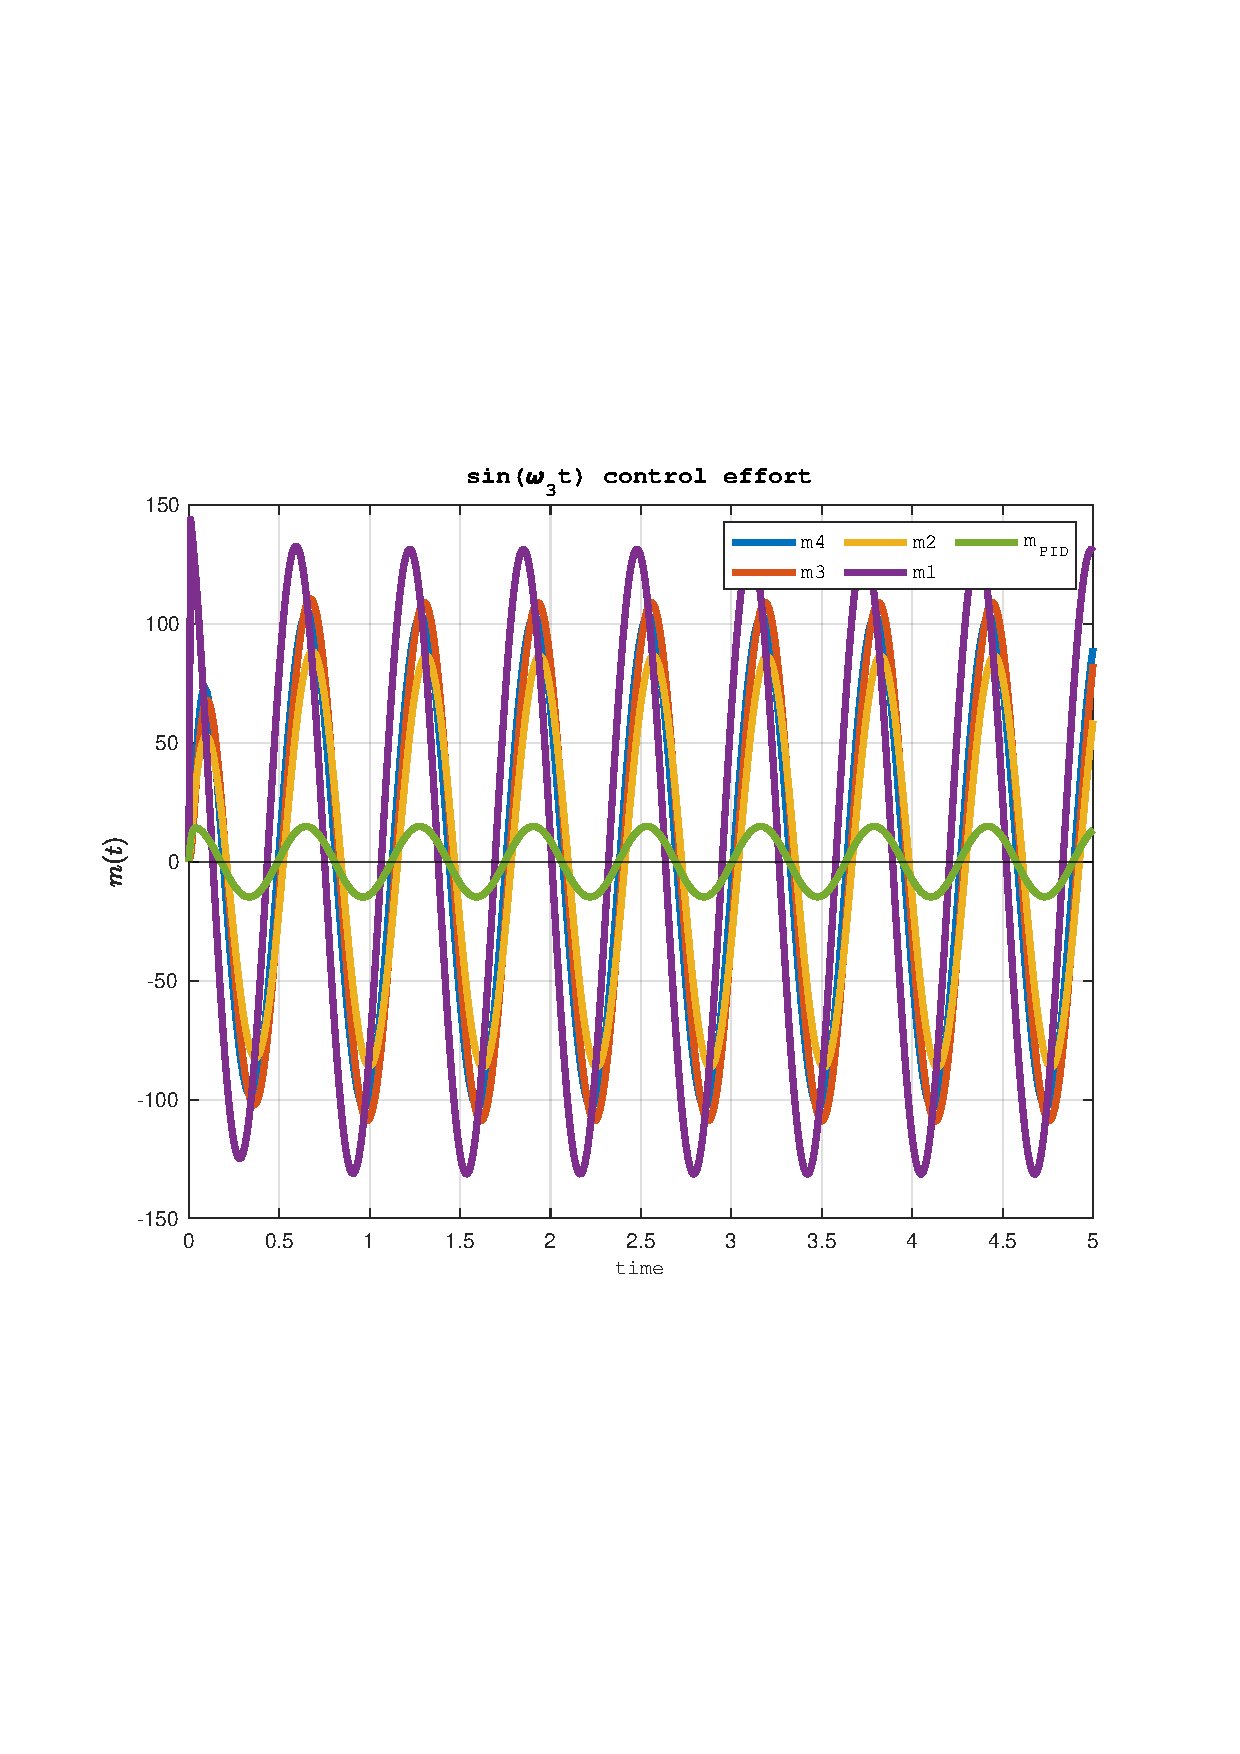
\includegraphics[width=\textwidth]{Figures/fig07f.pdf}
           \caption{Control effort for $\omega_3 = 10$}
           \label{fig:fig07f}
       \end{subfigure}
       \caption{Tracking and control effort w.r.t. sinusoidal references at different frequencies}
    \label{fig:fig07}
   \end{figure}

\clearpage
As shown in Fig.~\ref{fig:fig07} , the $H_\infty$ controllers start losing tracking accuracy already at $\omega_2 = 1$, due to phase shift (Fig. ). 
\\At lower frequencies, such as $\omega_1$, the tracking error is more than acceptable, with attenuation in module and phase shift both close to zero.\\\\
For $\omega_3 = 10$, attenuation starts to be relevant, but even more importantly, the phase shift hits the 90° mark (the output signal is in quadrature w.r.t the reference).
\\\\
The PID controller is clearly the wrong fit for the task: it can only track references at very low frequency. This is no surprise since with such a slow response time, it would be impossible to keep up with faster oscillations.\\
Its superiority in terms of control effort is therefore useless, since the tracking error is too large even at $\omega_1 = 1$.

\subsubsection{Conclusion - Problem 3}
For tracking a sinusoidal reference - at low frequency - the best controller is $C_1$. It still has the highest control effort demand among the group, but in this case, \textbf{considering only low frequency signals}, the difference is not so relevant. In exchange, it presents the lowest module attenuation and phase shift, and therefore is the right pick for this task.

\section{Problem 4: Measurement Noise}
The analysis so far has assumed no measurement noise in the loop. Let's remove this hypothesis and assume a random, high frequency noise that stays in the range $[-9\%,+9\%]$ of the signal maximum value (so for unitary references it will never exceed $\pm0.09$).\\\\
To simulate this scenario, I've used Simulink to generate the responses and Matlab to plot the results. 
The said data is available in the Folder "Data" and it can be generated any time through the Simulink file.
\\\\
Before looking at the plots, one can anticipate the system's behavior looking at the shape of the sensitivities. The PID, with its low bandwidth $T(s)$, is surely the most efficient in noise rejection.\\
Among the $H_\infty$ controllers, $C_4$ has the lowest bandwidth (being the only one with a complementary sensitivity weight $w_T$) and therefore should be slightly more robust w.r.t. noise rejection.

\begin{figure}[h!]
    \begin{subfigure}[t]{0.60\textwidth}
           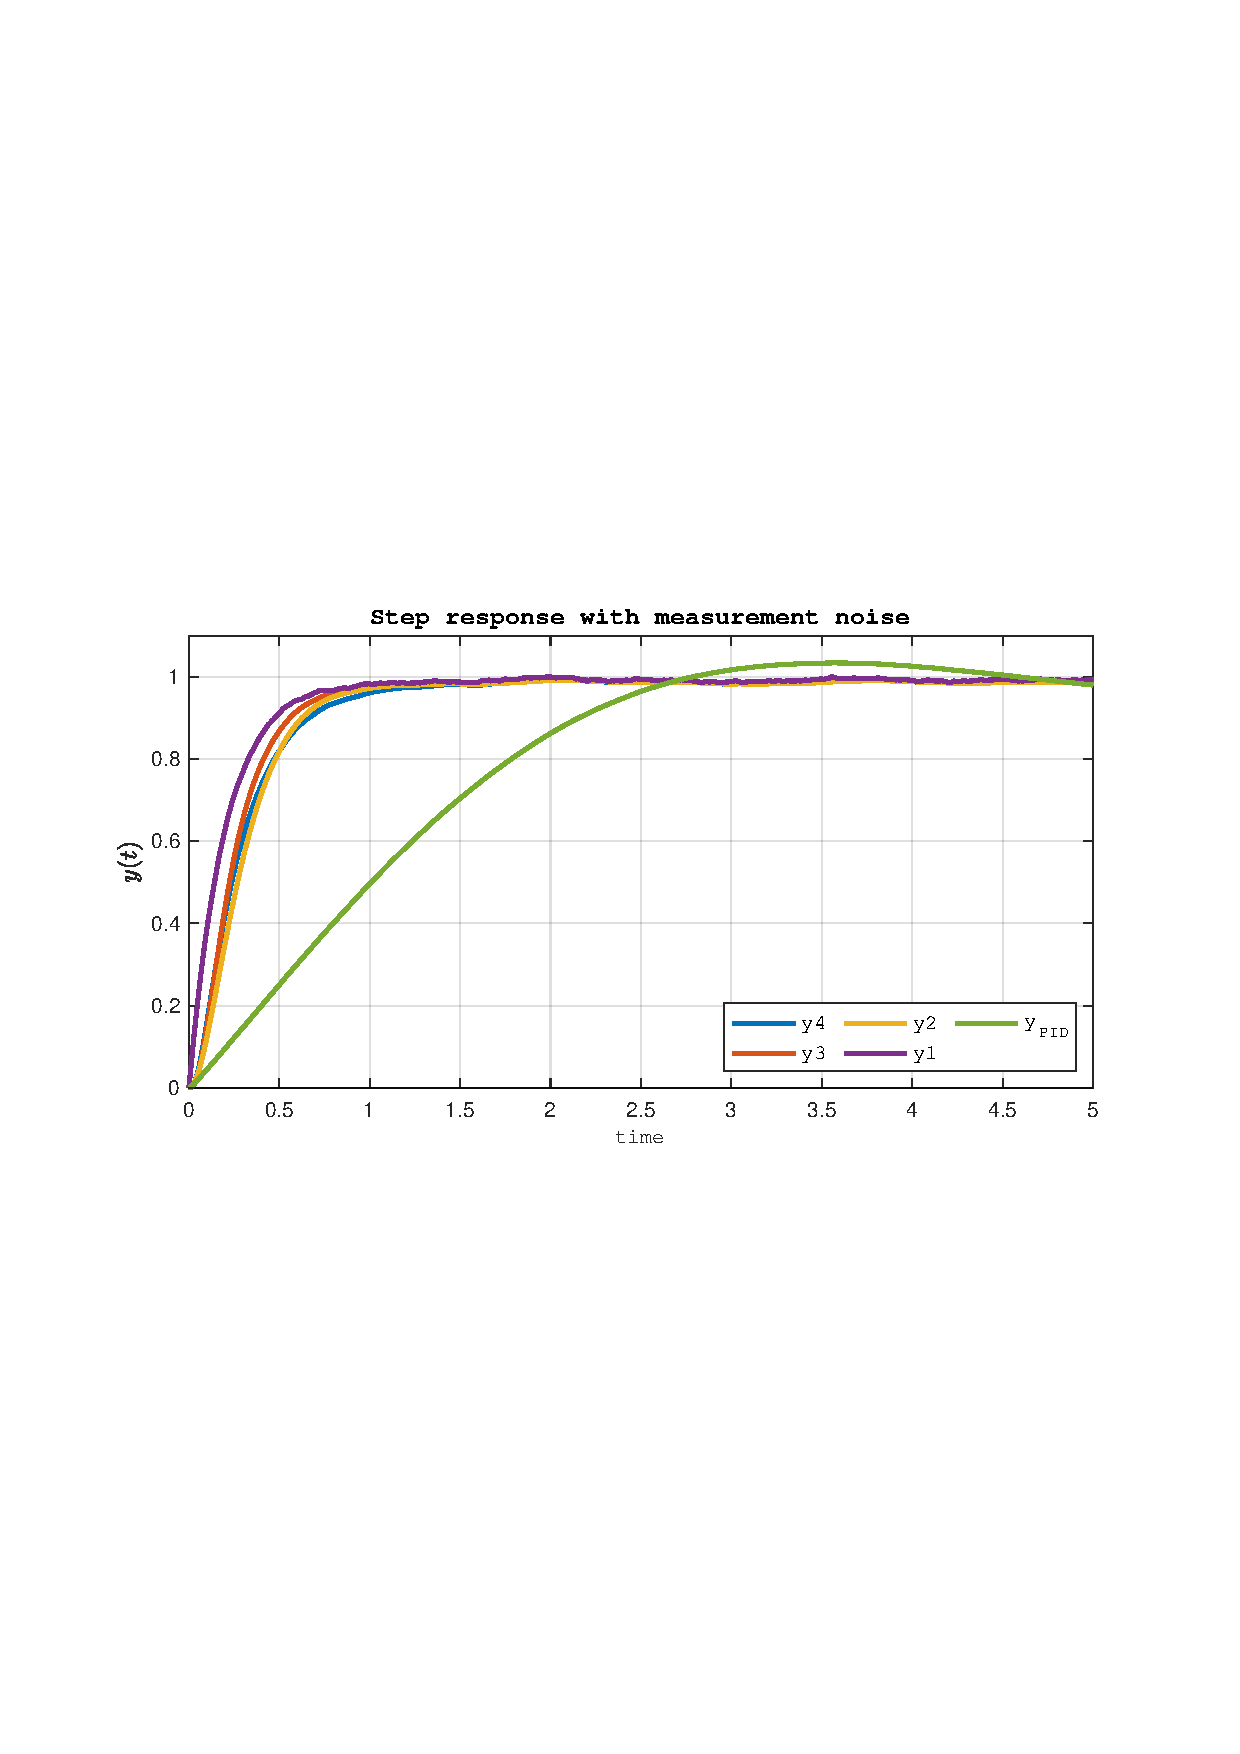
\includegraphics[width=\textwidth]{Figures/fig09a.pdf}
           \caption{Step response with n(t) $\neq$ 0}
           \label{fig:fig09a}
       \end{subfigure}
    \begin{subfigure}[t]{0.4\textwidth}
           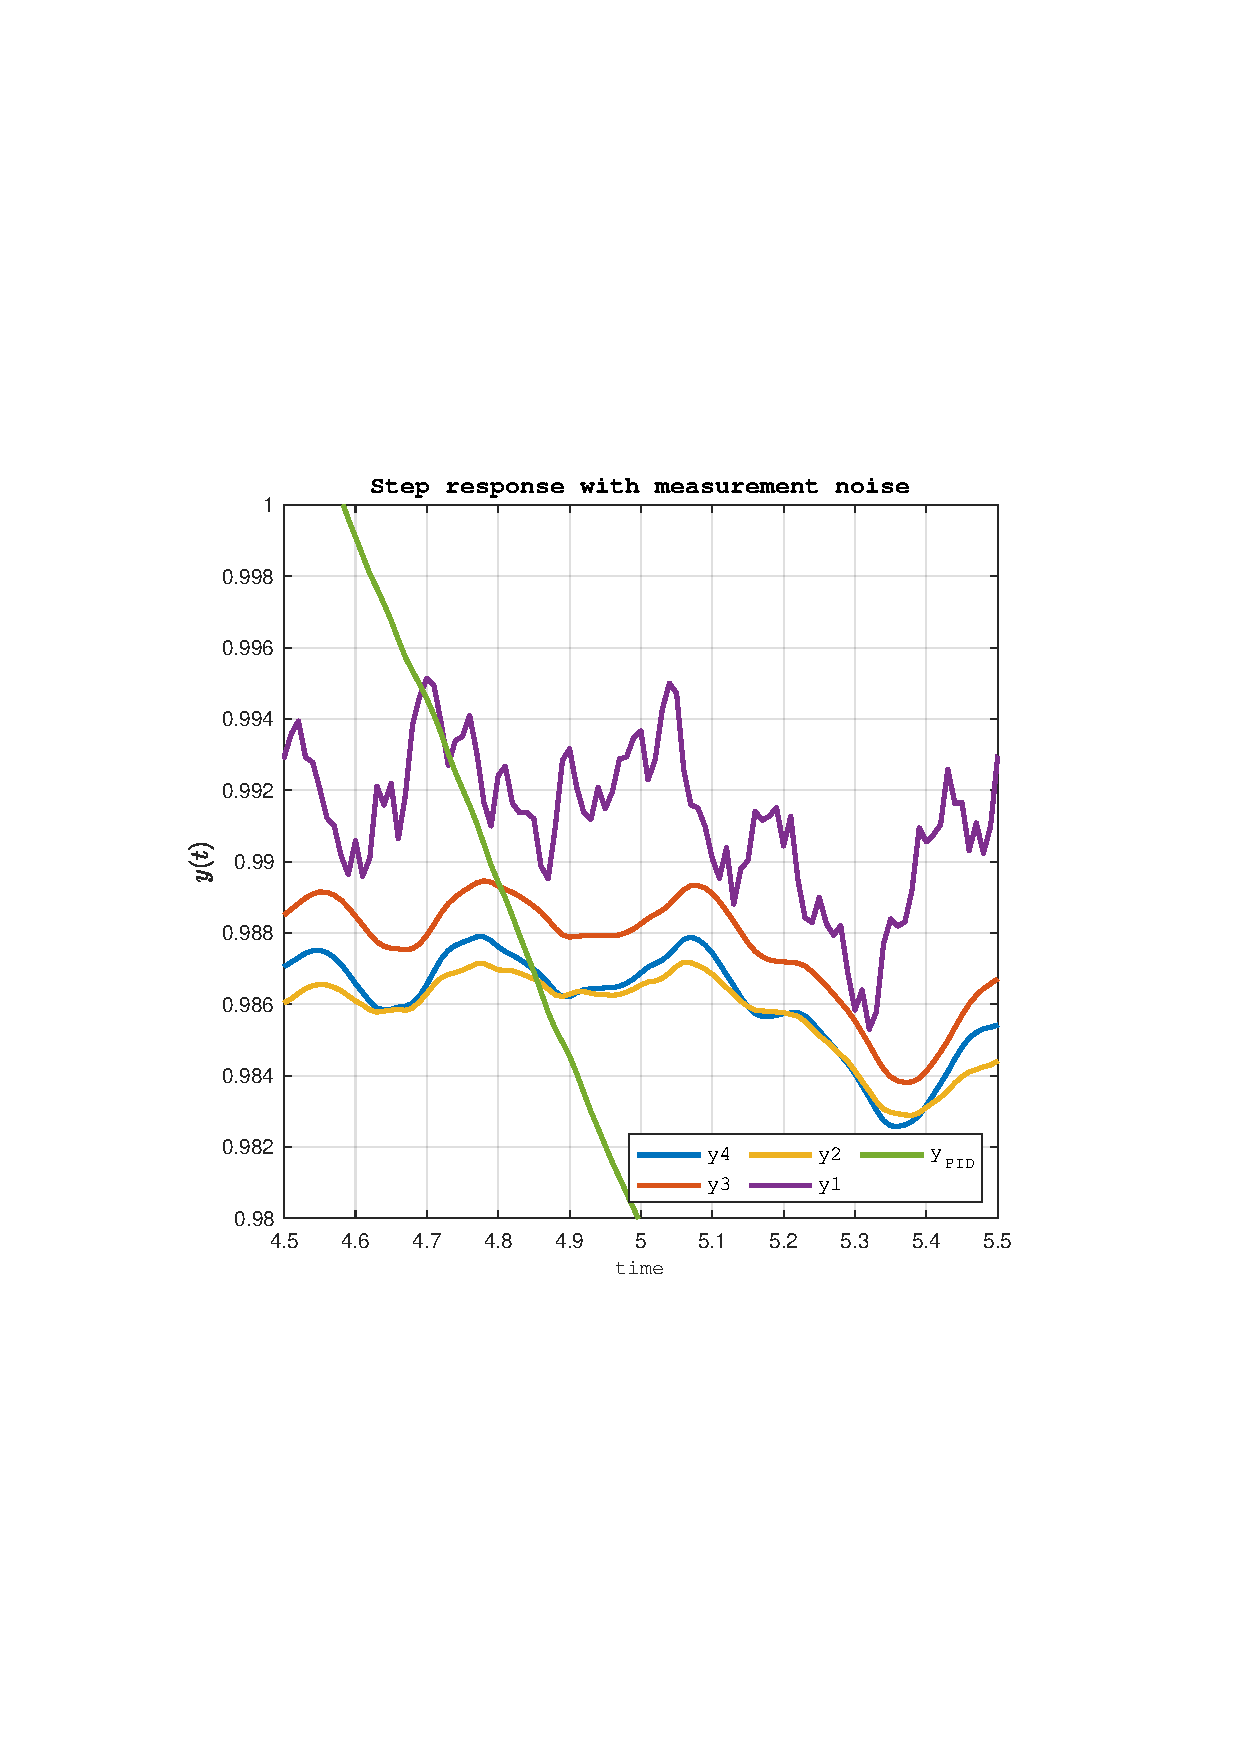
\includegraphics[width=\textwidth]{Figures/fig09b.pdf}
           \caption{Response zoom in}
           \label{fig:fig09b}
       \end{subfigure}
       \caption{Tracking of a step reference with random high frequency measurement noise}
    \label{fig:fig09}
   \end{figure}

Notice that also control effort will be susceptible to noise and in this sense, $C_3$ should be better performing, having the lowest $C_{S_u}$ bandwidth.
\begin{figure}[h!]
    \begin{subfigure}[t]{0.60\textwidth}
           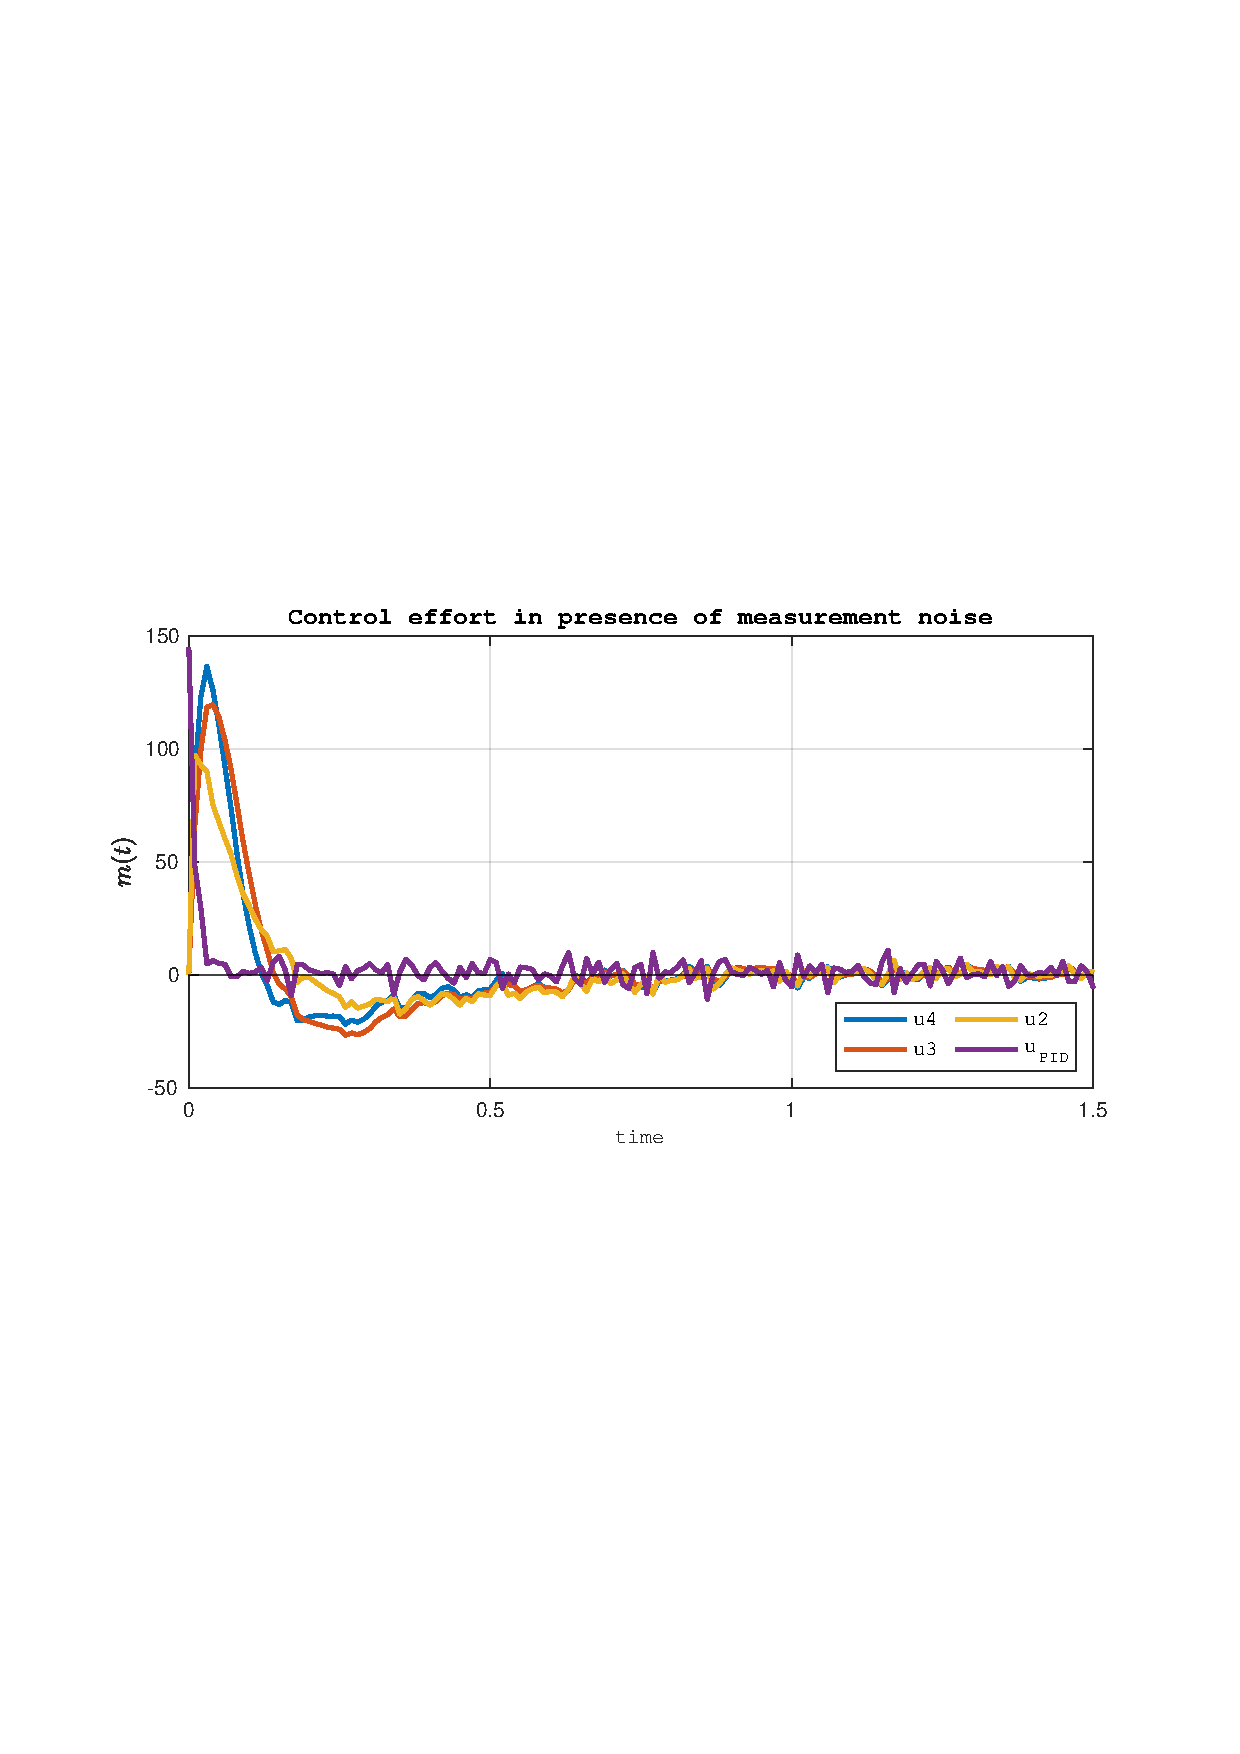
\includegraphics[width=\textwidth]{Figures/fig10a.pdf}
           \caption{Control effort with n(t) $\neq$ 0}
           \label{fig:fig10a}
       \end{subfigure}
    \begin{subfigure}[t]{0.4\textwidth}
           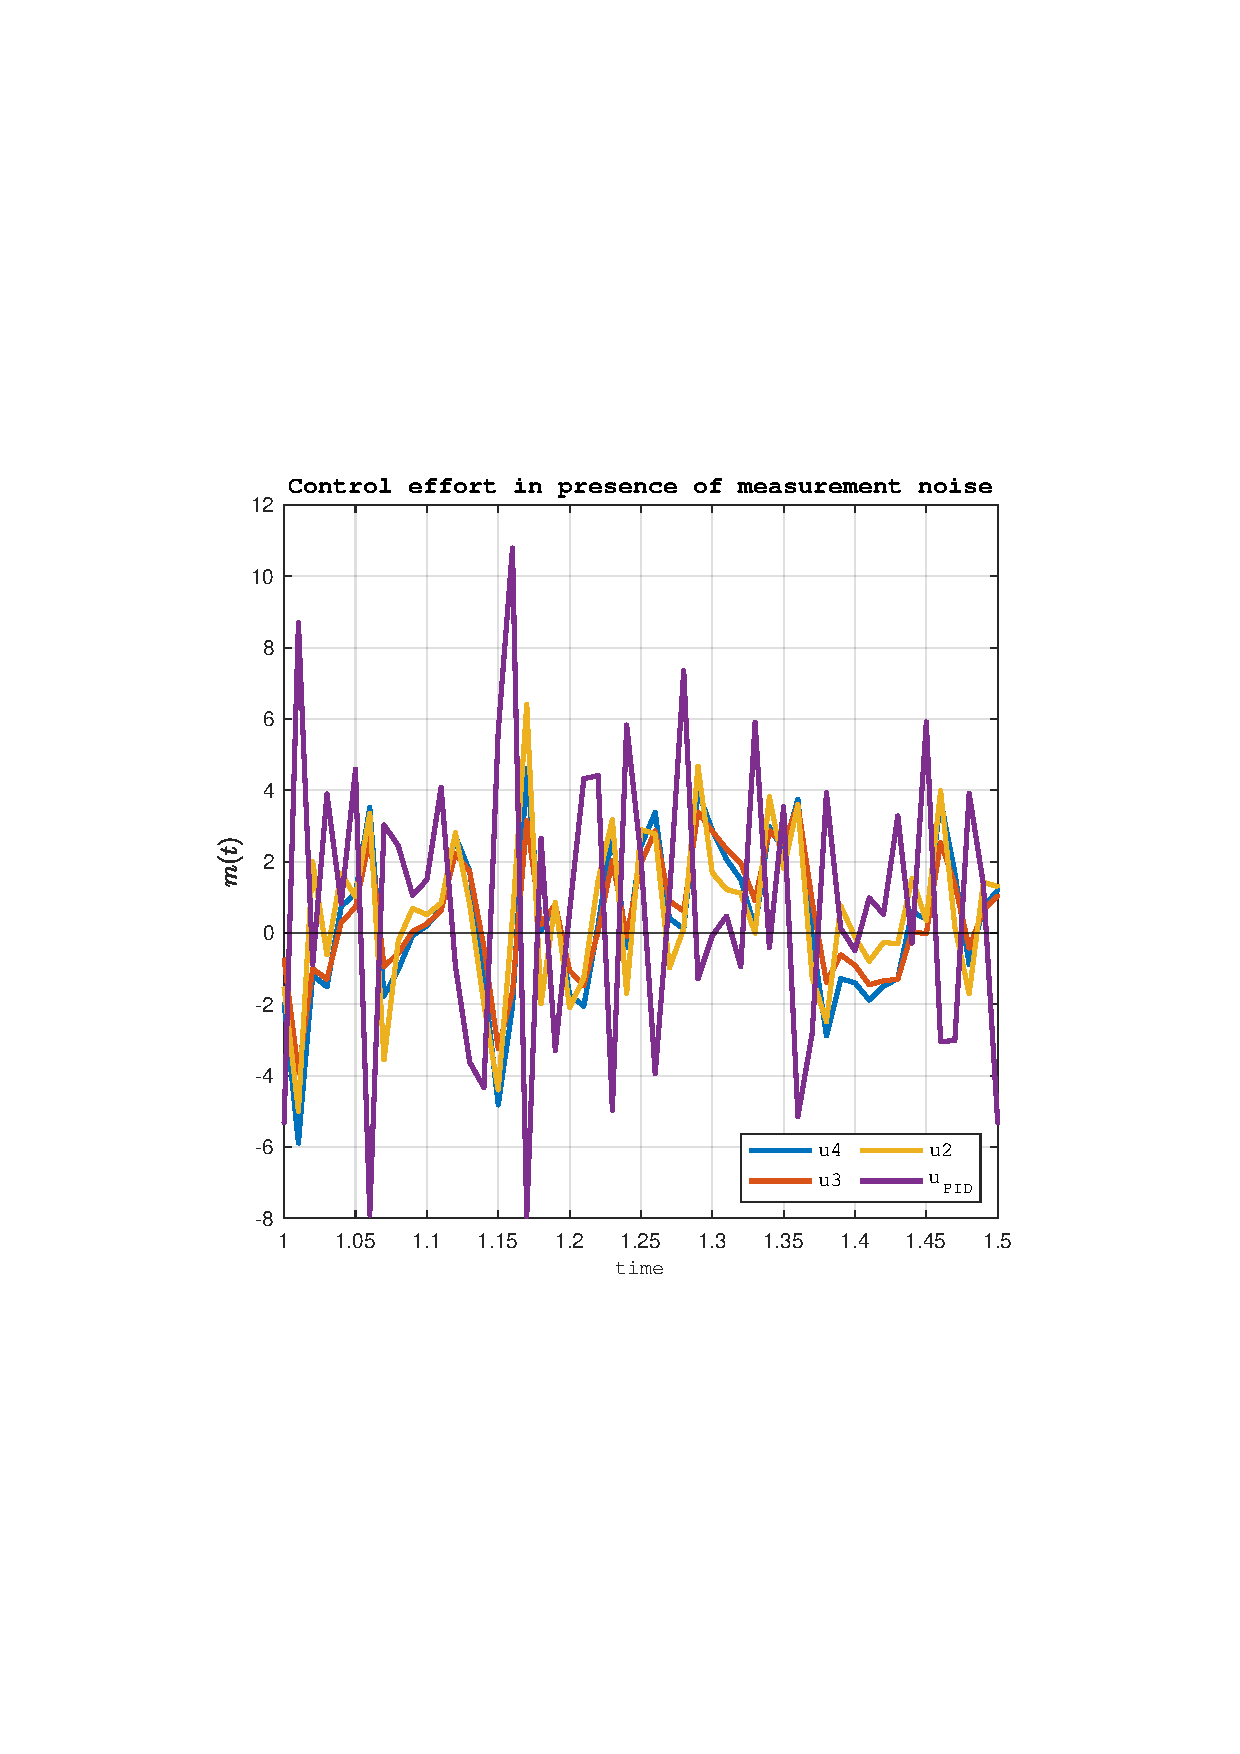
\includegraphics[width=\textwidth]{Figures/fig10b.pdf}
           \caption{Control effort zoom in}
           \label{fig:fig10b}
       \end{subfigure}
       \caption{Control effort to a step reference with random high frequency measurement noise}
    \label{fig:fig10}
   \end{figure}
\clearpage
\subsubsection{Conclusion - Problem 4}
In terms of pure noise rejection, the best performing controller is the PID. However, the tracking speed can't be put aside and so it's better to steer towards the $H_\infty$ controllers.\\\\
Unfortunately, the design so far has had the main goal of increasing bandwidth, and now it's time to pay the price.\\
For this reason, all controllers present discretely bad performance, especially in terms of control effort "spikiness".\\
That said, the controller $C_3$ offers the best compromise: less sensitive to noise in both response and control effort, with quite low tracking error.\\\\
However, it's clear that a 2-DoF control scheme that filters the feedback signal $y(t)-n(t)$ would be much more appropriate. As a matter of fact, it would not only further reduce the output noise, but more importantly it would cancel the "spikes" in the control effort, which are bad for any real world actuator (think of a DC motor).

\section{Problem 5: Double MSD system}
Let's now attach a second MSD system to the first Mass, still considering the output of the system to be the position of the first mass. The control input (acceleration for now) will be applied to the second mass this time.\\
The state equations become:
\begin{equation}
    \begin{bmatrix}
    \dot{x}_1 \\
    \dot{x}_2 \\
    \dot{x}_3 \\
    \dot{x}_4
    \end{bmatrix} =
    \begin{bmatrix}
    0 & 1 & 0 & 0 \\
    -\frac{k2+k1}{m_1} & -\frac{\mu_1+\mu_2}{m_1} &
    \frac{k_2}{m_1} & \frac{\mu_2}{m_1} \\
     0 & 0 & 0 & 1 \\
    \frac{k_2}{m_2} & \frac{\mu_2}{m_2} &
    -\frac{k_2}{m_2} & -\frac{\mu_2}{m_2} \\
    \end{bmatrix}
    \begin{bmatrix}
    x_1 \\
    x_2 \\
    x_3 \\
    x_4
    \end{bmatrix} +
    \begin{bmatrix}
    0\\
    0\\
    0\\
    \frac{1}{m_2}
    \end{bmatrix}
    u(t)\ \ \ \ 
    y(t) = x_1
\end{equation}
We expect some noticeable oscillatory behavior, which will get worse the lower the damping coefficients. The bode magnitude plot confirms this intuition presenting of a very large peak. Therefore, \textbf{the main focus for our design will be mitigating oscillations} in the transient, even if that means sacrificing bandwidth.
\\
Tuning the sensitivity weights as in the Matlab file, the resulting $H_\infty$ controller is very performing. In particular, through the sensitivity weight, I required a tracking error under 1\%, also "squishing" the peak and mitigating the oscillations. I chose a constant control sensitivity weight to limit the magnitude of the $S_u(j\omega)$. Comparing the obtained controller with a classic PIDF controller, the difference is staggering. Oscillations are completely annihilated and the transient time has been lowered from 90s to about 4.5s.
\\Of course the price for this performance increase comes in terms of control effort and robustness with respect to noise. One could mitigate both effects by decreasing bandwidth and coping with an higher transient time. However, for eliminating the oscillations some kind of compensation is still required, hence some "sacrifices" in terms of control effort must always be taken into account. .\\
Fig.~\ref{fig:fig11} shows comparisons between step response and control effort for both the PID-contolled and the $H_\infty$ one.
\begin{figure}[h!]
 \begin{subfigure}[t]{0.45\textwidth}
    \includegraphics[width=\textwidth]
    {Figures/fig11a.pdf}
    \captionsetup{margin=2mm}
    \caption{Step response with $H_\infty$ controller}
    \label{fig:fig11a}
    \end{subfigure}
    \begin{subfigure}[t]{0.45\textwidth}
       \includegraphics[width=\textwidth]
       {Figures/fig11b.pdf}
       \captionsetup{margin=2mm}
       \caption{Step response with $PID$ controller}
       \label{fig:fig03b}
   \end{subfigure}
   \begin{subfigure}[t]{0.50\textwidth}
       \includegraphics[width=\textwidth]
       {Figures/fig11c.pdf}
       \captionsetup{margin=2mm}
       \caption{Step control effort for $H_\infty$ controller}
       \label{fig:fig11c}
   \end{subfigure}
    \begin{subfigure}[t]{0.5\textwidth}
       \includegraphics[width=\textwidth]
       {Figures/fig11d.pdf}
       \captionsetup{margin=2mm}
       \caption{Step control effort for $PID$ controller}
       \label{fig:fig11d}
   \end{subfigure}
   \caption{Step response comparison between $H_\infty$ and PID}
       \label{fig:fig11}
\end{figure}
\clearpage
\subsection{Conclusion - Problem 5}
Adding a second mass introduces a large peak in the plant's Bode Magnitude plot, which is symptom of oscillatory behavior during transient. The presence of damping guarantees asymptotic stability and also "shortens" the time of oscillation, which inversely proportional to the damping coefficient. 
\\\\The main goal of our controller's design has therefore been eliminating the oscillations, possibly reducing the transient time.\\
\\Notice that despite increased dimensionality, the system is still minimum phase, which allows us to perform "hardcore" $H_\infty$ control: plant ($P(s)$) cancellation and new dynamics' assignment.
\\ \\
That's the exact reason why the $H_\infty$ controller designed with the chosen sensitivity weights outperforms the PIDF controller by such a long shot. \\While the PIDF has to cope with the slow, highly oscillating dynamics of the plant, the $H_\infty$ cancels out the whole plant and assigns a new - faster and non-oscillating - one.
\\\\
We know for sure that this method is not robust with respect to parametric uncertainty, but for such a simple system one can assume a good knowledge of the parameters that can guarantee effectiveness of the controller.

\section{Problem 6: Double MSD system with DC Motor}
Let's now consider a front wheel actuation on the second mass, provided by a DC motor. In this case, the control input $u(t)$ becomes the Voltage $V(t)$ whereas the output of the system is still the position of the first mass (unactuated). We consider the motor current as the state variable $x_5$ and select the motor's parameters in a consistent way.\\   
Hence, under pure-rolling assumptions, the state the state equations become:
\begin{equation}
    \begin{bmatrix}
    \dot{x}_1 \\
    \dot{x}_2 \\
    \dot{x}_3 \\
    \dot{x}_4\\
    \dot{x}_5
    \end{bmatrix} =
    \begin{bmatrix}
    0 & 1 & 0 & 0 & 0\\
    -\frac{k2+k1}{m_1} & -\frac{\mu_1+\mu_2}{m_1} &
    \frac{k_2}{m_1} & \frac{\mu_2}{m_1} & 0\\
     0 & 0 & 0 & 1 & 0\\
    \frac{k_2}{m_2} & \frac{\mu_2}{m_2} &
    -\frac{k_2}{m_2} & -\frac{\mu_2}{m_2} & 
    \frac{K_t}{m_2r}\\
     0 & 0 & 0 & \frac{K_e}{L} &-\frac{R}{Lr}
    \end{bmatrix}
    \begin{bmatrix}
    x_1 \\
    x_2 \\
    x_3 \\
    x_4 \\
    x_5
    \end{bmatrix} +
    \begin{bmatrix}
    0\\
    0\\
    0\\
    0\\
    \frac{1}{Lr}
    \end{bmatrix}
    u(t)\ \ \ \ 
    y(t) = x_1
\end{equation}
\\Even with increased dimentionality and much worse open loop performance, the system is still stable and minimum phase, which allows us to per form "hardcore" $H_\infty$ control with plant cancellation and new dynamics' assignment.
\\ To do that, let's first examine what the main goal of our control design should be. Fig.~\ref{fig:fig12} shows a highly oscillating transient, due to the low frequency complex poles. Moreover, the Plant converges at the desired position in about 200 seconds, which is a ridiculously long time.
\begin{figure}[h!]
    \centering
    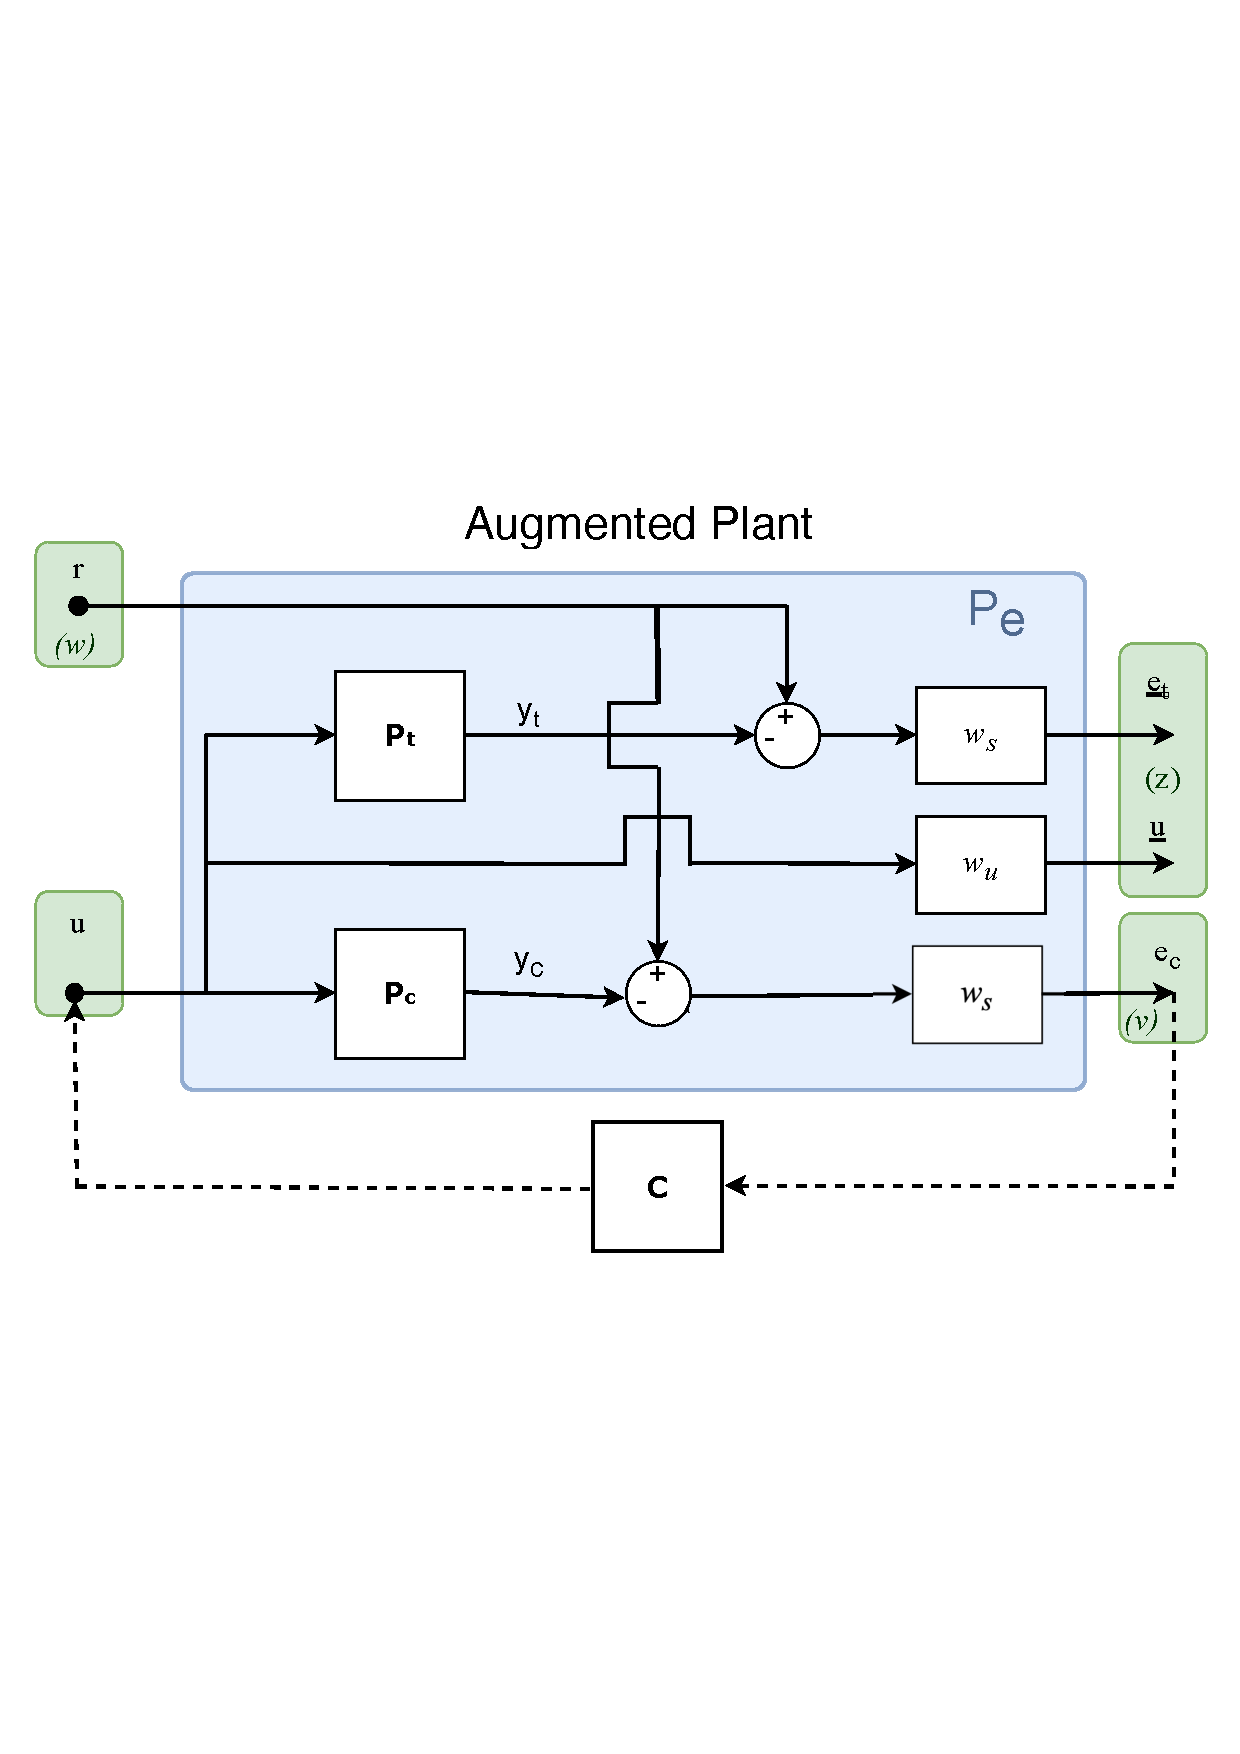
\includegraphics[width=\textwidth]
    {Figures/fig12.pdf}
        \caption{Open Loop Position Tracking}
    \label{fig:fig12}
\end{figure}

Since we're dealing with a DC motor, the \textbf{main goal of our control design will be keeping the Voltage (input $u(t)$) into a safe operating range, while mitigating the oscillations}. In this case we'll sacrifice bandwidth in order to prioritize these other requirements.
\\\\
This time, the Control Sensitivity weight $w_{S_u}(s)$ is deigned as a transfer function with the following aims:
\begin{enumerate}
    \item Limit control effort in magnitude
    \item Limit high-pass behaviors that can cause control effort peaks when dealing with step references
\end{enumerate}
The Sensitivity weight instead $w_S(s)$ has the purpose of:
\begin{enumerate}
    \item Bound tracking error at a maximum of 1\%
    \item Mitigate, if not annihilate, all oscillations
\end{enumerate}
Figure Fig.~\ref{fig:fig13} shows that through $H_\infty$ control (and importantly, through plant cancellation) we achieve a almost perfect tracking of the step reference - with no oscillations or overshoot whatsoever - in about 7 seconds, nothing compared to the open loop 200 seconds.
\begin{figure}[h!]
    \centering
    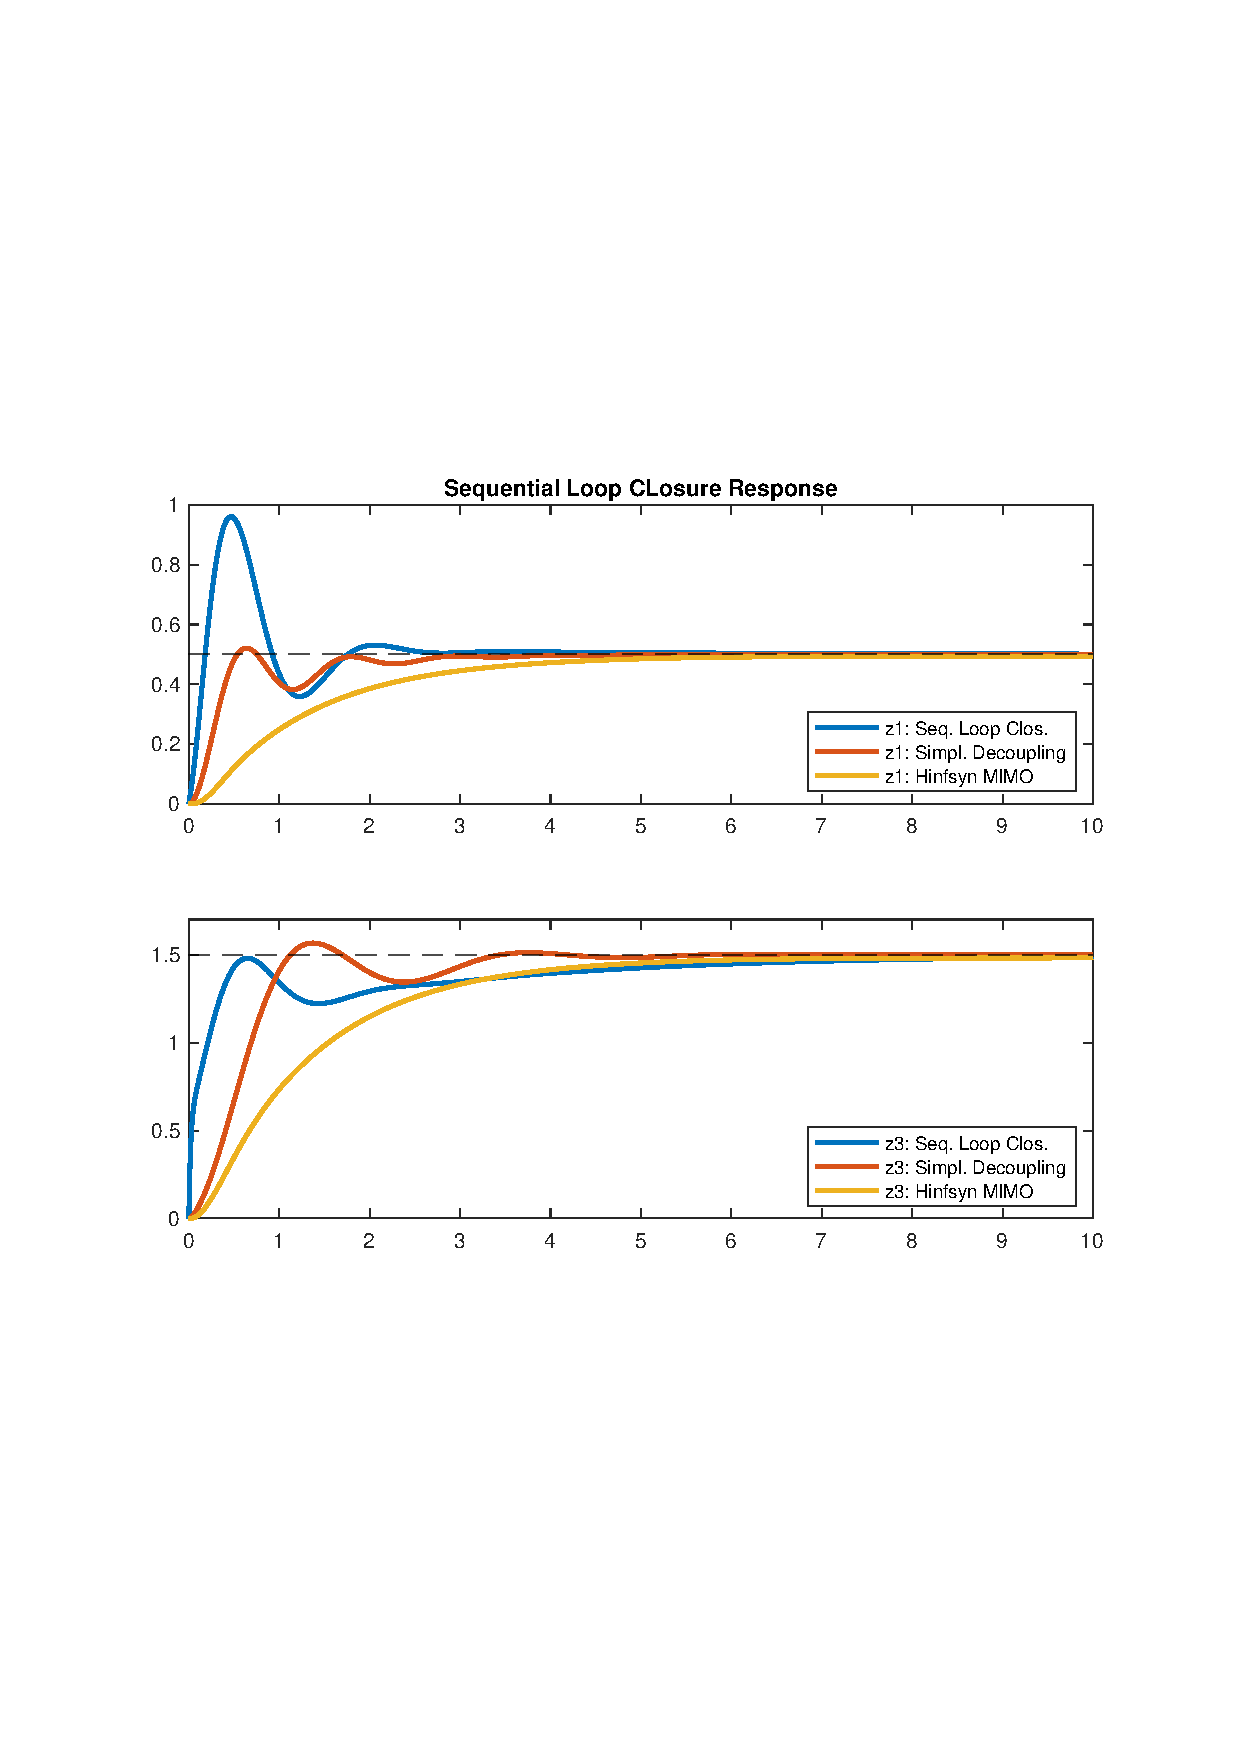
\includegraphics[width=0.8\textwidth]
    {Figures/fig13.pdf}
        \caption{$H_\infty$ Position Tracking}
    \label{fig:fig13}
\end{figure}
\\
The control effort (in this case, the armature voltage) (Fig.~\ref{fig:fig14}) is kept at more than reasonable levels. The system is still "sensitive" to references with high frequency content, but the control effort in module stays bounded in an acceptable range of Voltage, realistically not causing any saturation of the motor.
\begin{figure}[h!]
    \centering
    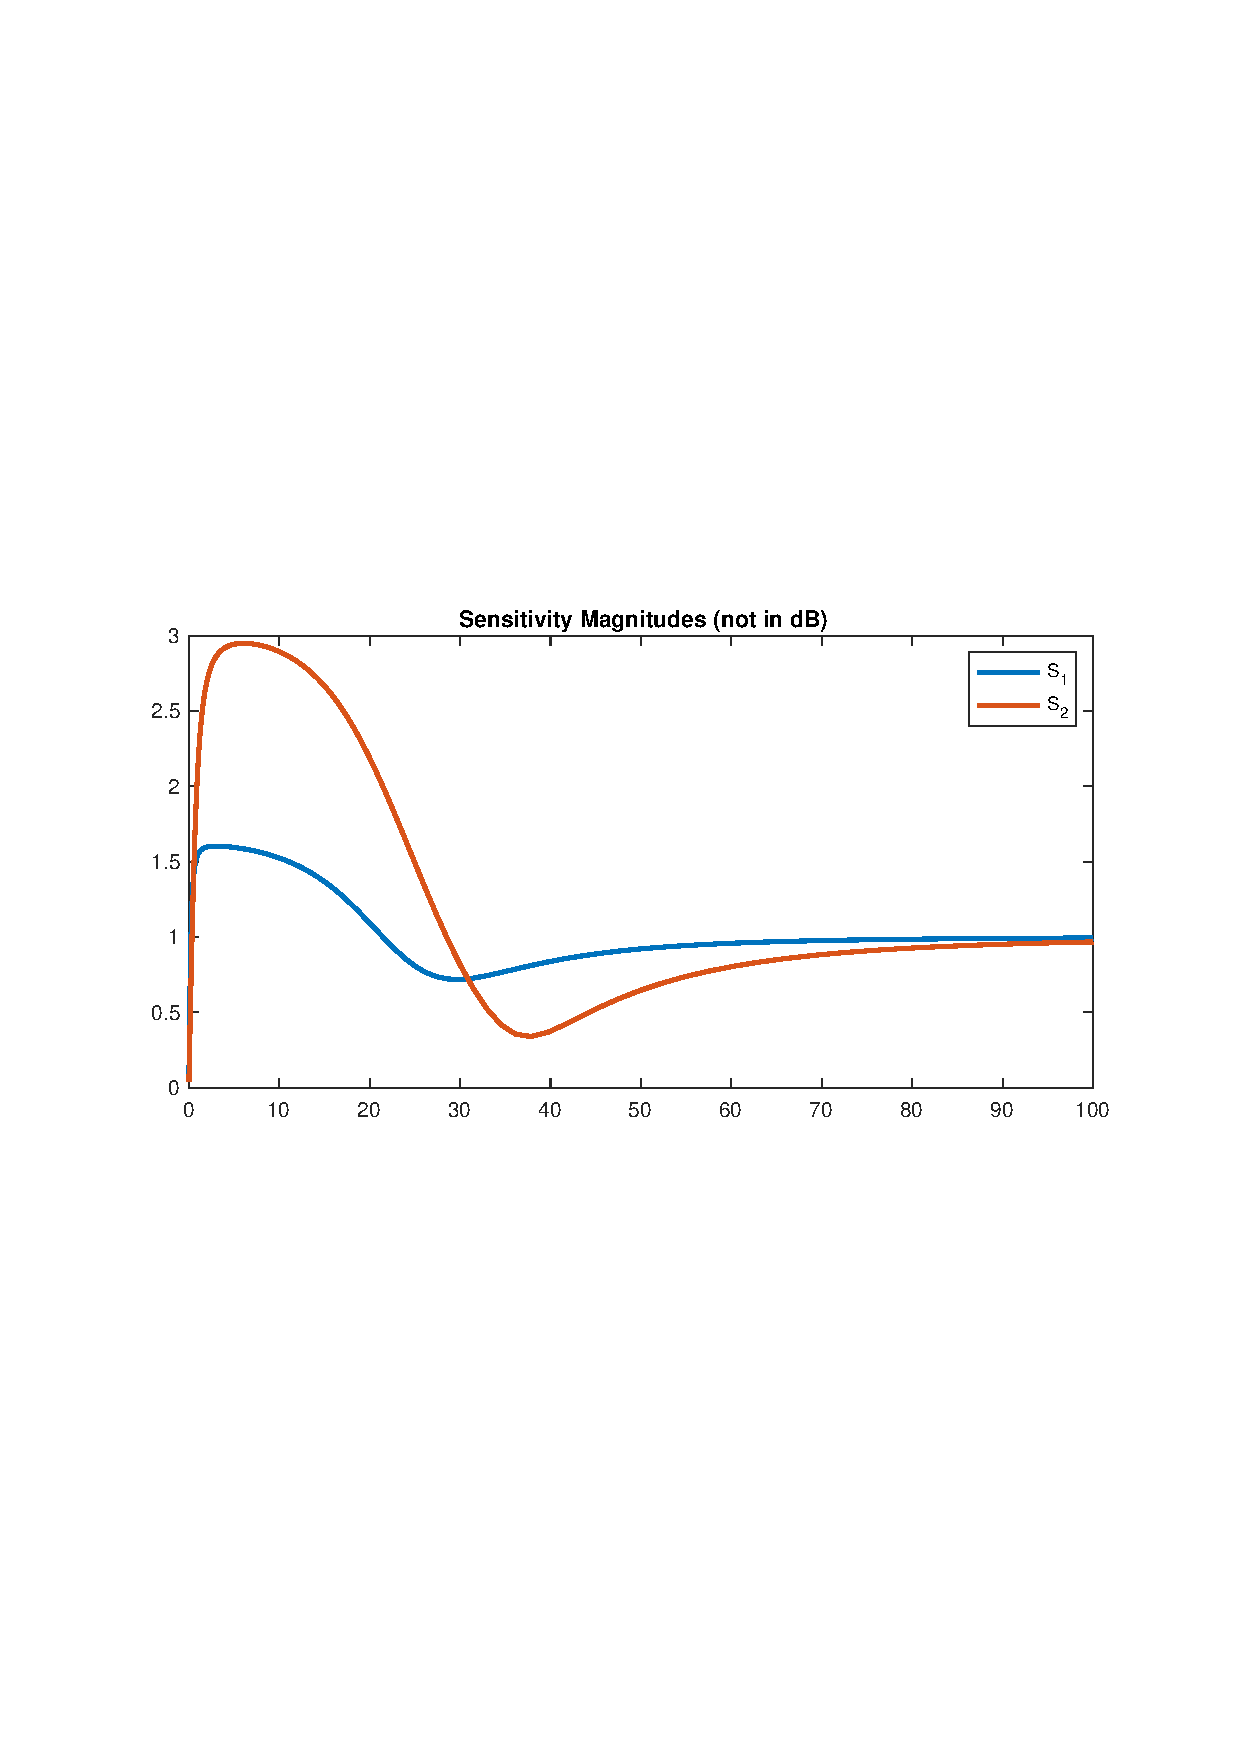
\includegraphics[width=0.8\textwidth]
    {Figures/fig14.pdf}
        \caption{$H_\infty$ Voltage control effort}
    \label{fig:fig14}
\end{figure}
\\
\end{document}

